
\documentclass[a4paper,11pt]{article}%,twocolumn
%% packages

\usepackage{blindtext} % needed for creating dummy text passages
%\usepackage{ngerman} % needed for German default language
\usepackage{amsmath} % needed for command eqref
\usepackage{amssymb} % needed for math fonts
\usepackage[colorlinks=true,breaklinks]{hyperref} % needed for creating hyperlinks in the document, the option colorlinks=true gets rid of the awful boxes, breaklinks breaks lonkg links (list of figures), and ngerman sets everything for german as default hyperlinks language
\usepackage[hyphenbreaks]{breakurl} % ben�tigt f�r das Brechen von URLs in Literaturreferenzen, hyphenbreaks auch bei links, die �ber eine Seite gehen (mit hyphenation).
\usepackage{xcolor}
\definecolor{c1}{rgb}{0,0,1} % blue
\definecolor{c2}{rgb}{0,0.3,0.9} % light blue
\definecolor{c3}{rgb}{0.3,0,0.9} % red blue
\hypersetup{
    linkcolor={c1}, % internal links
    citecolor={c2}, % citations
    urlcolor={c3} % external links/urls
}
%\usepackage{cite} % needed for cite
\usepackage[square,authoryear]{natbib} % needed for cite and abbrvnat bibliography style
\usepackage[nottoc]{tocbibind} % needed for displaying bibliography and other in the table of contents
\usepackage{graphicx} % needed for \includegraphics 
\usepackage{longtable} % needed for long tables over pages
\usepackage{bigstrut} % needed for the command \bigstrut
\usepackage{enumerate} % needed for some options in enumerate
%\usepackage{todonotes} % needed for todos
\usepackage{makeidx} % needed for creating an index
\makeindex
\usepackage{gensymb}
\usepackage{url}
\usepackage{psfrag}
\usepackage{multirow}
\usepackage{subfigure}
%% page settings

\usepackage[top=20mm, bottom=20mm,left=15mm,right=15mm]{geometry} % needed for page border settings
\parindent=0mm % for space of first line of new text block
\sloppy % for writing with hyphenless justification (tries to)
\hyphenation{} % use hyphenation of tolerance parametershttp://www.jr-x.de/publikationen/latex/tipps/zeilenumbruch.html
\hyphenpenalty=10000
\exhyphenpenalty=10000
\usepackage{fancyhdr} % needed for head and foot options
%% my macros

%% Text fomats
\newcommand{\tbi}[1]{\textbf{\textit{#1}}}

%% Math fonts
\newcommand{\bbA}{\mathbb{A}}
\newcommand{\bbB}{\mathbb{B}}
\newcommand{\bbC}{\mathbb{C}}
\newcommand{\bbD}{\mathbb{D}}
\newcommand{\bbE}{\mathbb{E}}
\newcommand{\bbF}{\mathbb{F}}
\newcommand{\bbG}{\mathbb{G}}
\newcommand{\bbH}{\mathbb{H}}
\newcommand{\bbI}{\mathbb{I}}
\newcommand{\bbJ}{\mathbb{J}}
\newcommand{\bbK}{\mathbb{K}}
\newcommand{\bbL}{\mathbb{L}}
\newcommand{\bbM}{\mathbb{M}}
\newcommand{\bbN}{\mathbb{N}}
\newcommand{\bbO}{\mathbb{O}}
\newcommand{\bbP}{\mathbb{P}}
\newcommand{\bbQ}{\mathbb{Q}}
\newcommand{\bbR}{\mathbb{R}}
\newcommand{\bbS}{\mathbb{S}}
\newcommand{\bbT}{\mathbb{T}}
\newcommand{\bbU}{\mathbb{U}}
\newcommand{\bbV}{\mathbb{V}}
\newcommand{\bbW}{\mathbb{W}}
\newcommand{\bbX}{\mathbb{X}}
\newcommand{\bbY}{\mathbb{Y}}
\newcommand{\bbZ}{\mathbb{Z}}
\usepackage[ framed, numbered]{matlab-prettifier}%framed,%
\usepackage{listings}
\usepackage{physics}
\usepackage{pdfpages}
\usepackage[toc,page]{appendix}
\usepackage{float}
% for code
\usepackage{listings}
\usepackage{color}
\usepackage{pifont}

\usepackage{scalerel,xparse}
\NewDocumentCommand\emojismile{}{
    \scalerel*{
        
\includegraphics{./figures/emoji/u1F62C.png}
    }{X}
}


% Define colors
\definecolor{codegreen}{rgb}{0,0.6,0}
\definecolor{codegray}{rgb}{0.5,0.5,0.5}
\definecolor{codepurple}{rgb}{0.58,0,0.82}
\definecolor{backcolour}{rgb}{0.95,0.95,0.92}
% Setup the listings package
\lstset{
    backgroundcolor=\color{backcolour},   
    commentstyle=\color{codegreen},
    keywordstyle=\color{magenta},
    numberstyle=\tiny\color{codegray},
    stringstyle=\color{codepurple},
    basicstyle=\footnotesize,
    breakatwhitespace=false,         
    breaklines=true,                 
    captionpos=b,                    
    keepspaces=true,                 
    numbers=left,                    
    numbersep=5pt,                  
    showspaces=false,                
    showstringspaces=false,
    showtabs=false,                  
    tabsize=2
}



\begin{document}
\begin{titlepage}
\center % Center everything on the page

%-------------------------------------------------------------------------------------
%	HEADING SECTIONS
%------------------------------------------------------------------------------------
\textbf{\large Department of Electrical and Computer Engineering}\\[0.5cm]
\textbf{\Large University of Colorado at Boulder}\\[1cm]
\textbf{\large ECEN5823 - Low Power Embedded Design Techniques}\\[2cm]

\includegraphics[width=0.3\textwidth]{figures/cu}\\[2cm] 

	
%-------------------------------------------------------------------------------------
%	TITLE SECTION
%------------------------------------------------------------------------------------
\textbf{\Huge Spring 2024, ECEN 5823 }\\[0.2cm]

\textbf{\Large Course Project Report}\\[5cm]


%----------------------------------------------------------------------------------------
%	MEMBERS SECTION
%----------------------------------------------------------------------------------------


\vfill

\textbf{\large Submitted by}

{\large Parth Thakkar}\\[0.5cm]

%----------------------------------------------------------------------------------------
%	DATE SECTION
%----------------------------------------------------------------------------------------

\textbf{\large Submitted on}\\
\textbf{\Large \today} % Date, change the \today to a set date if you want to be precise

%----------------------------------------------------------------------------------------

\vfill % Fill the rest of the page with whitespace

\end{titlepage}

\pagebreak

\tableofcontents
\listoffigures
\listoftables
\vfill
\begin{center}
    \textbf{\textit{*PDF is clickable}}
\end{center}

\pagebreak

% \section{}

\section{\color{red}Project Proposal}



\textbf{Team name:}\\
Low Self Esteem Team\\

\textbf{Student Name:}\\
Parth Rajeshkumar Thakkar\\
ParthRajeshkumar.Thakkar@colorado.edu\\

Anagha Aditya\\
Anagha.Aditya@colorado.edu\\

Akash Karoshi\\
Akash.Karoshi@colorado.edu\\


\subsection{Project Rationale and Goals}
For the ECEN 5833 Low Power Embedded System Design course, our team is developing an advanced mechanical keyboard called "The Insane Keyboard". This project aims to create a high-performance input device that combines ergonomic design, customization options, and some cool features.


\subsubsection{Project Rationale}
Our analysis of the mechanical keyboard market revealed several issues:
\begin{itemize}
    \item Ergonomic keyboards often lack additional features or are expensive
    \item Many feature-rich keyboards are wired, limiting mobility
    \item Affordable keyboards offer limited customization
    \item Few keyboards combine ergonomic design, wireless capability, programmable lighting, and smart functions
    \item Keyboards with displays or extra features often have poor power efficiency
\end{itemize}
\subsubsection{Project Goals}
We aim to create a mechanical keyboard with the following features:
\begin{itemize}
    \item Split ergonomic design to reduce physical strain
    \item Wireless connectivity using Bluetooth Low Energy.
    \item Programmable RGB lighting with addressable LEDs
    \item Hot-swappable key switches for easy customization
    \item Low-power E-ink display for additional information
    \item Multi-device compatibility
    \item Advanced power management techniques
    \item Environment temperature and pressure sensing.
    \item Real Time clock module for timer, stopwatch and time features.
    \item Potential energy harvesting from typing (Yet to be seen)
    \item Open-source firmware for extensive customization
    \item Cost-effective design for market accessibility
\end{itemize}

\subsubsection{Unique Features}
"The Insane Keyboard" has unique features like:
\begin{itemize}
    \item Integration of multiple desirable features in one device
    \item Optimized power management for extended use
    \item Potential energy harvesting from typing motions
    \item Open-source firmware for community-driven development
    \item Adaptable design for future upgrades
\end{itemize}

\subsubsection{Expected Outcomes}
Upon completion, this project could:
\begin{itemize}
    \item Improve ergonomics in daily computer use
    \item Advance keyboard power management and energy harvesting
    \item Foster a community of keyboard enthusiasts and developers
    \item Demonstrate practical applications of low-power embedded design
\end{itemize}

\subsection{Existing Products and Ideas from products}

% Placeholder for a diagram of the keyboard design
\begin{figure}[H]
    \centering
    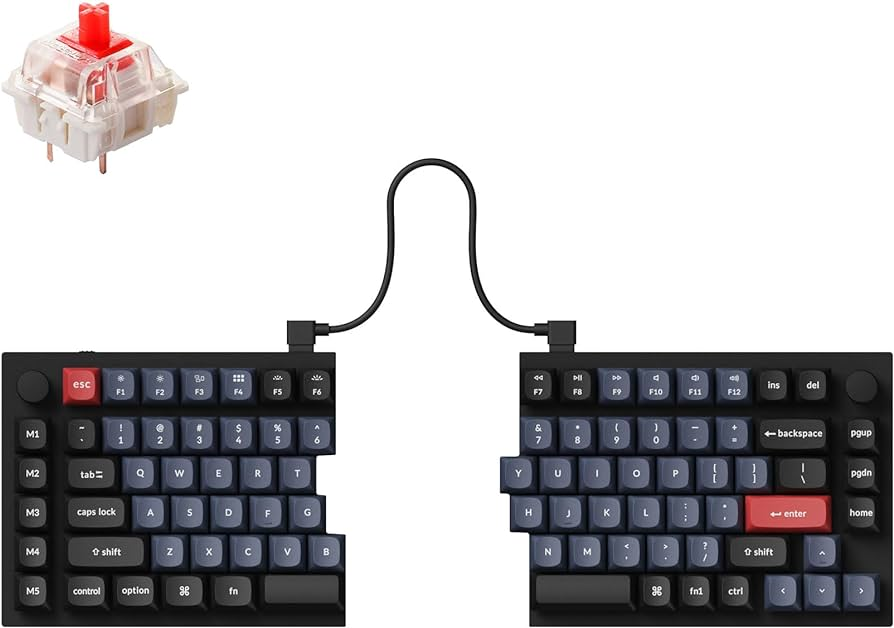
\includegraphics[scale=0.53]{figures/split_keyboard.jpg}
    \caption{Split Keyboard without display(Wired)}
    % Figure content to be added
\end{figure}
\vspace{0.2cm}
\begin{figure}[H]
    \centering
    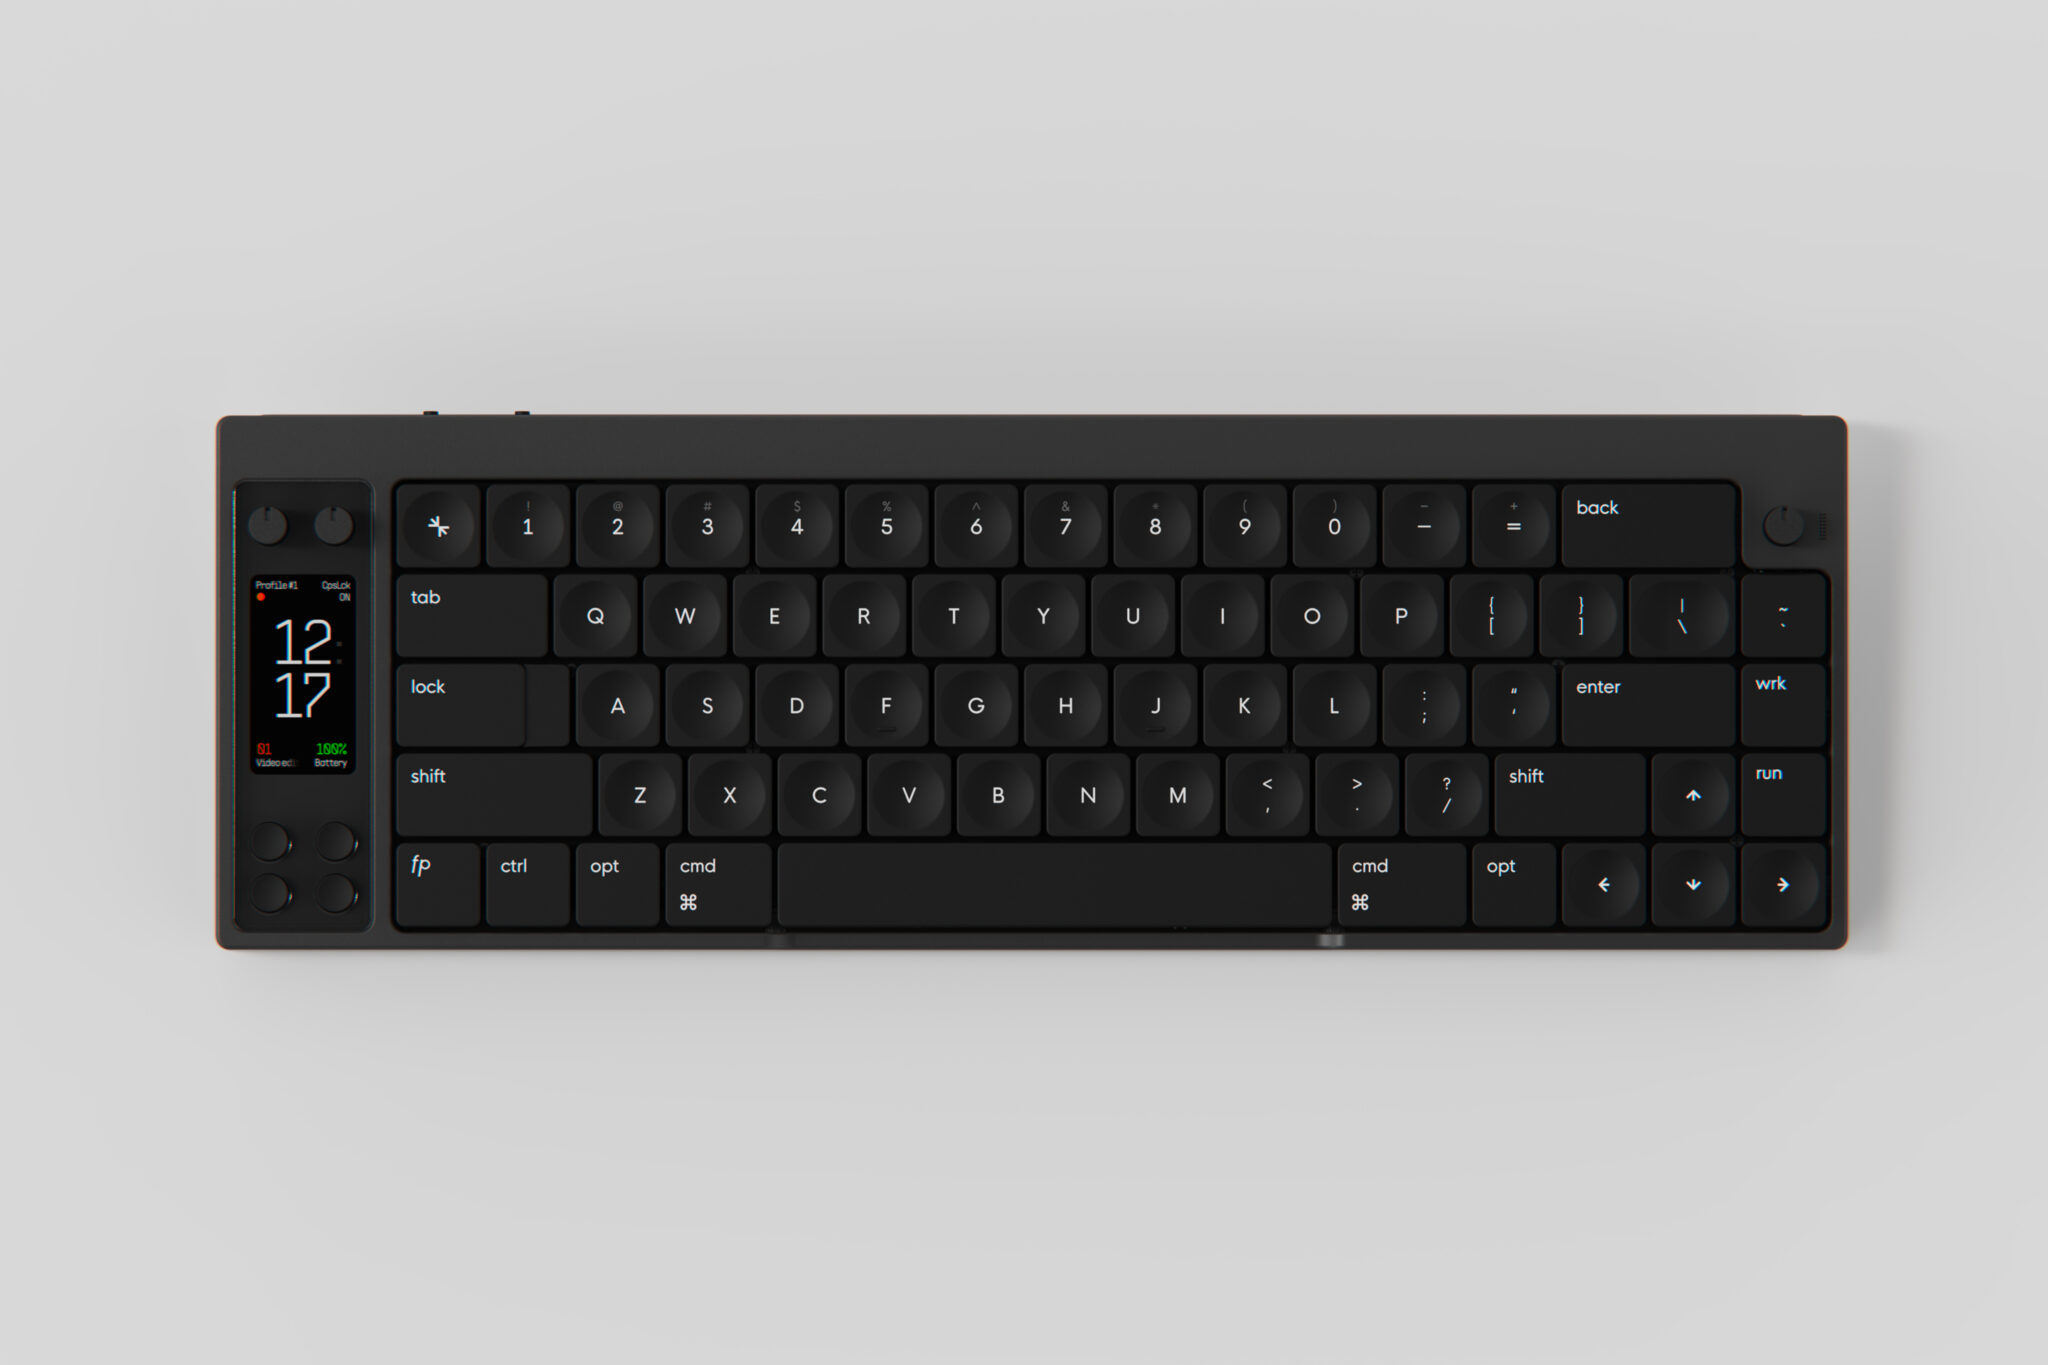
\includegraphics[scale=0.26]{figures/nomad.jpg}
    \caption{Keyboard which is expensive and have a Display}
    % Figure content to be added
\end{figure}
\vspace{0.2cm}

\begin{figure}[H]
    \centering
    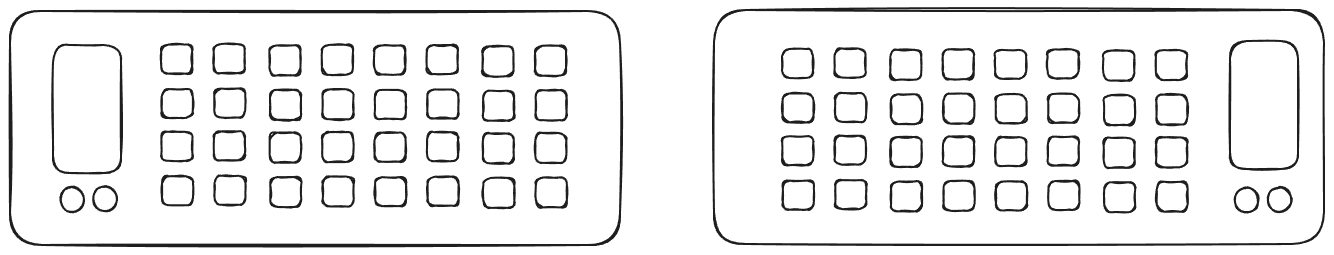
\includegraphics[scale=0.38]{figures/concept.png}
    \caption{Conceptual Design of The Insane Keyboard}
    % Figure content to be added
\end{figure}
\vspace{0.2cm}





\subsection{High Level Requirements}


\subsubsection{General Requirements}
\begin{itemize}
\item Two EFR32BG13 boards (one per module)
\item Should be Ergonomic
\item 75\% keyboard layout (TKL layout)
\item IO expander for each MCU
\item Temperature sensor
\item Pressure sensor
\item Real-Time Clock (RTC)
\item Connectivity to three host devices
\item Computer software for LED customization
\item Individually customizable LEDs
\item E-ink display on each module
\item Energy harvesting on each module
\item Charging circuit with Type-C connector
\item Charging indicator
\item Battery indicator
\item Minimum 6-key rollover
\item HID protocol communication between modules
\item Smart power states (active, idle, deep sleep)
\item RTOS: FreeRTOS (Yet to be decide)
\item PWM-based RGB LED control
\item Hot-swappable key switches
\item Time, date, battery status, current profile, custom graphics
\item Spotify integration for music control and now-playing information(yet to be seen)
\end{itemize}


    
\subsection{Keyboard Layout and Design}

\subsubsection{Main Board Key Layout}
\begin{center}
\begin{tabular}{|c|c|c|c|c|c|c|}
\hline
\multicolumn{7}{|c|}{\textbf{Function Row}} \\ \hline
\begin{tabular}[c]{@{}c@{}}ESC\ $\sim$ `{}\end{tabular} &
\begin{tabular}[c]{@{}c@{}}F1\ 1 !\end{tabular} &
\begin{tabular}[c]{@{}c@{}}F2\ 2 @\end{tabular} &
\begin{tabular}[c]{@{}c@{}}F3\ 3 \#\end{tabular} &
\begin{tabular}[c]{@{}c@{}}F4\ 4 \$\end{tabular} &
\begin{tabular}[c]{@{}c@{}}F5\ 5 \%\end{tabular} &
\begin{tabular}[c]{@{}c@{}}F6\ 6 \^{}\end{tabular} \\
\hline
\multicolumn{7}{|c|}{\textbf{QWERTY Row}} \\
\hline
TAB & Q & W & E & R & T &\\
\hline
\multicolumn{7}{|c|}{\textbf{Home Row}} \\
\hline
CAPS & A & S & D & F & G & \\
\hline
\multicolumn{7}{|c|}{\textbf{Bottom Row}} \\
\hline
SHIFT & Z & X & C & V & B & \\
\hline
\multicolumn{7}{|c|}{\textbf{Modifier Row}} \\
\hline
CTRL & OPT & WIN/MAC & ALT & \multicolumn{3}{c|}{SPACE} \\
\hline
\end{tabular}
\end{center}
\textbf{Additional Inputs:}
\begin{itemize}
\item 2 × Rotary Encoders (Knobs)
\item 3 × Extra Buttons
\end{itemize}
\textbf{Additional Components}
\begin{itemize}
    \item E-Ink display
    \item Battery
    \item Battery Charging and Power Management Unit \textcolor{yellow}{(Not in Secondary module)}
    \item Tempurature Sensor \textcolor{yellow}{(Not in Secondary module)}
    \item Real time Clock \textcolor{yellow}{(Not in Secondary module)}
\end{itemize}

\subsection{Secondary Module Key Layout}
\begin{center}
\begin{tabular}{|c|c|c|c|c|c|c|c|}
\hline
\multicolumn{8}{|c|}{\textbf{Function Row}} \\
\hline
F7 & F8 & F9 & F10 & F11 & F12 & BKSP & HOME \\
\hline
\multicolumn{8}{|c|}{\textbf{QWERTY Row}} \\
\hline
Y & U & I & P & \{[ & \}] & |$\backslash$  & DEL \\
\hline
\multicolumn{8}{|c|}{\textbf{Home Row}} \\
\hline
H & J & K & L & \begin{tabular}[c]{@{}c@{}}; :\end{tabular} & \begin{tabular}[c]{@{}c@{}}" '\end{tabular} & ENTER & PGUP \\
\hline
\multicolumn{8}{|c|}{\textbf{Bottom Row}} \\
\hline
N & M & \begin{tabular}[c]{@{}c@{}}, <\end{tabular} & \begin{tabular}[c]{@{}c@{}}. >\end{tabular} & \begin{tabular}[c]{@{}c@{}}/ ?\end{tabular} & SHIFT & ↑ & PGDN \\
\hline
\multicolumn{8}{|c|}{\textbf{Modifier Row}} \\
\hline
& SPACE & ALT/MAC & FN & CTRL & ← & ↓ & → \\
\hline
\end{tabular}
\end{center}
\textbf{Additional Inputs:}
\begin{itemize}
\item 2 × Rotary Encoders (Knobs)
\item 3 × Extra Buttons
\end{itemize}
\textbf{Additional Components:}
\begin{itemize}
    \item E-Ink display
    \item Battery
    \item Power Management Unit
\end{itemize}


\subsection{Challenges and Considerations}
\begin{itemize}
\item Managing state machines with complex software like e-ink display drivers
\item Integrating drivers with BLE firmware
\item Implementing RTC driver and temperature control driver
\item Ensuring reliable wireless connectivity
\item Implementing multi-host communication and switching
\item Developing HID profile in BLE stack
\item Implementing anti-ghosting techniques
\item Optimizing keyboard scan rate for low latency
\item Achieving N-key rollover or 6-key rollover
\end{itemize}

\pagebreak
\section{\color{red}Project Update: Week 1}



\subsection{Technical Considerations}


\subsubsection{Functional hardware block diagram}

\begin{figure}[H]
    \centering
    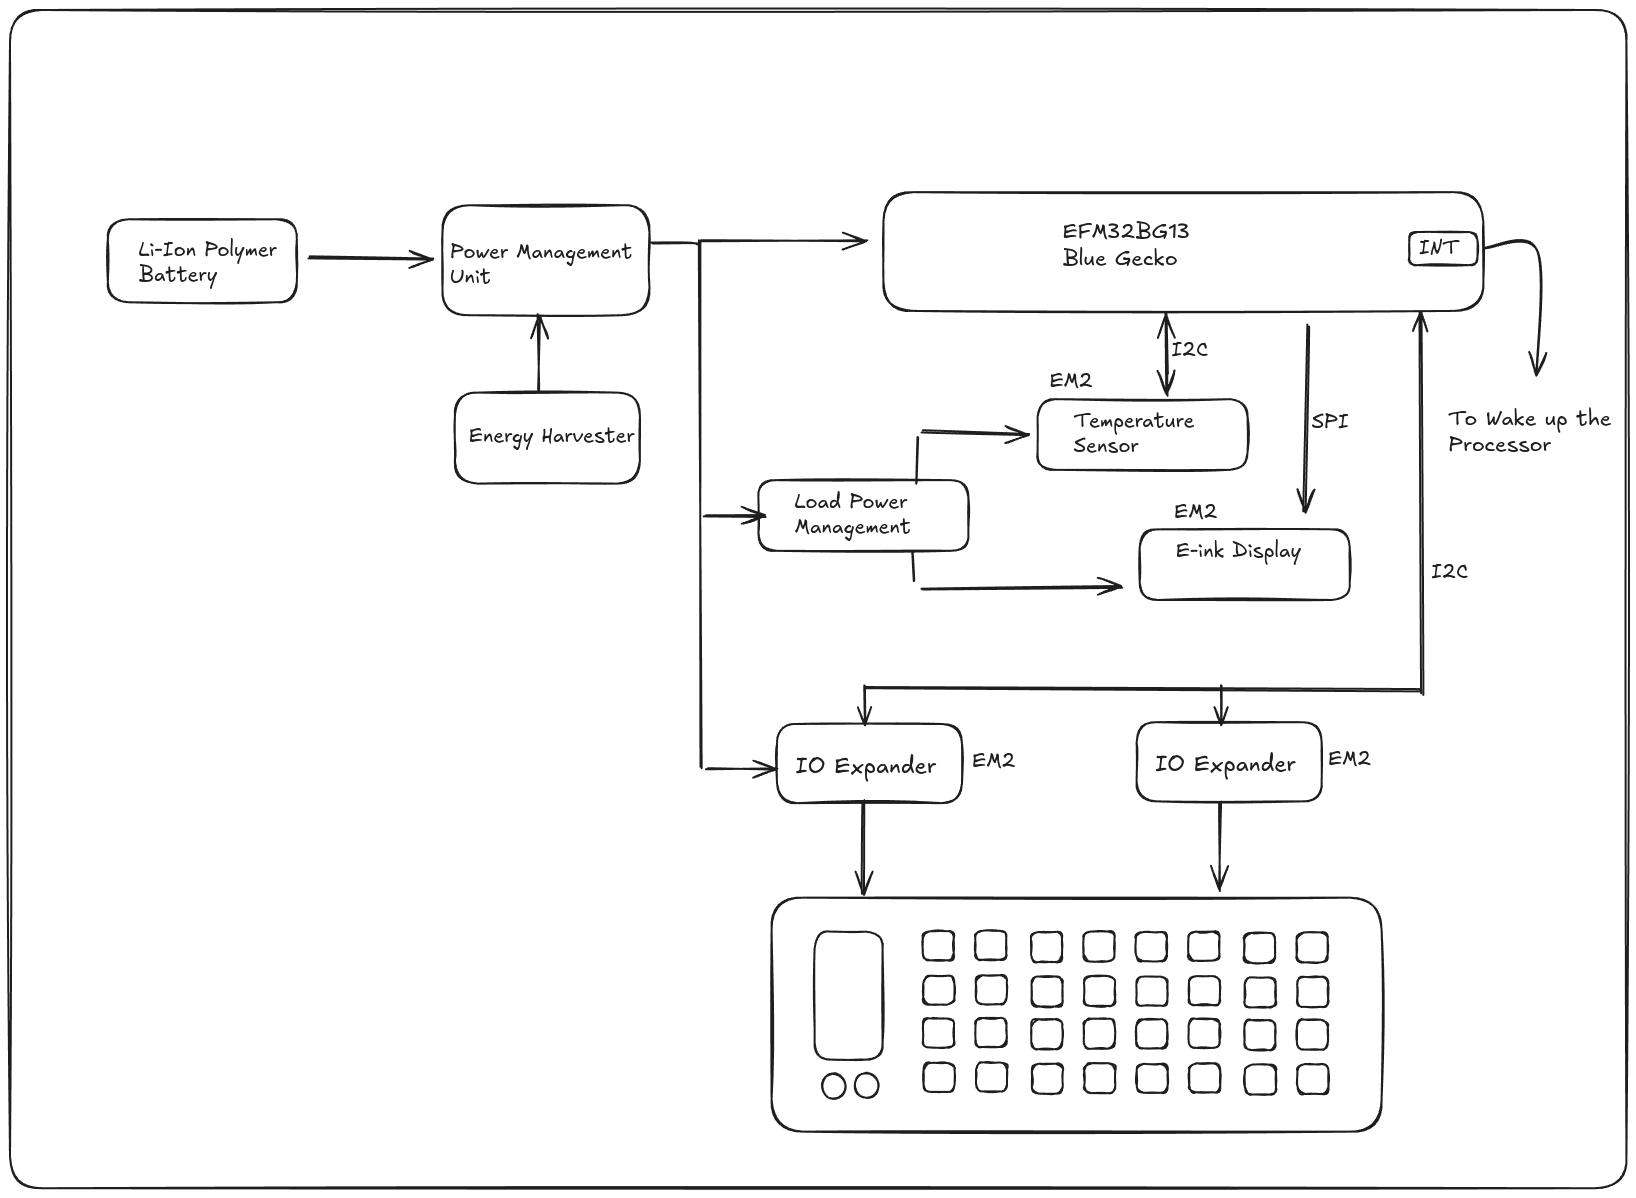
\includegraphics[scale=0.32]{figures/blockdiagram.png}
    \caption{Hardware block diagram}
    % Figure content to be added
\end{figure}
\vspace{0.2cm}


\textbf{0-Key Rollover (Normal Matrix)}
\begin{figure}[H]
	\centering
	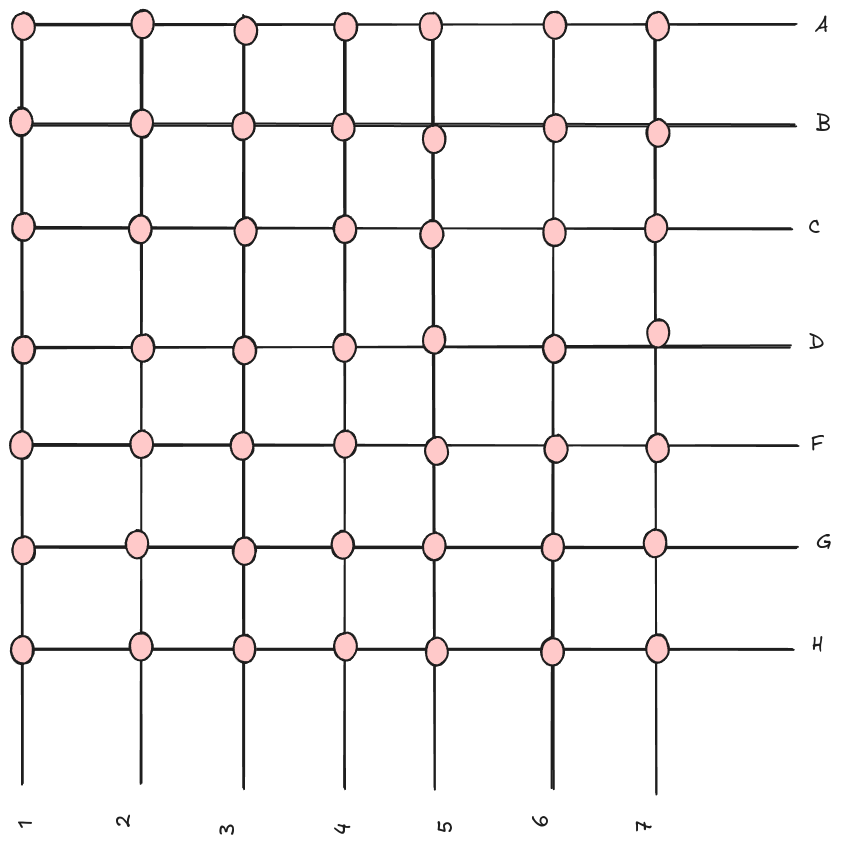
\includegraphics[scale=0.6]{figures/NRO.png}
	\caption{Normal Matrix for no key roll over}
\end{figure}
\begin{figure}[H]
	\centering
	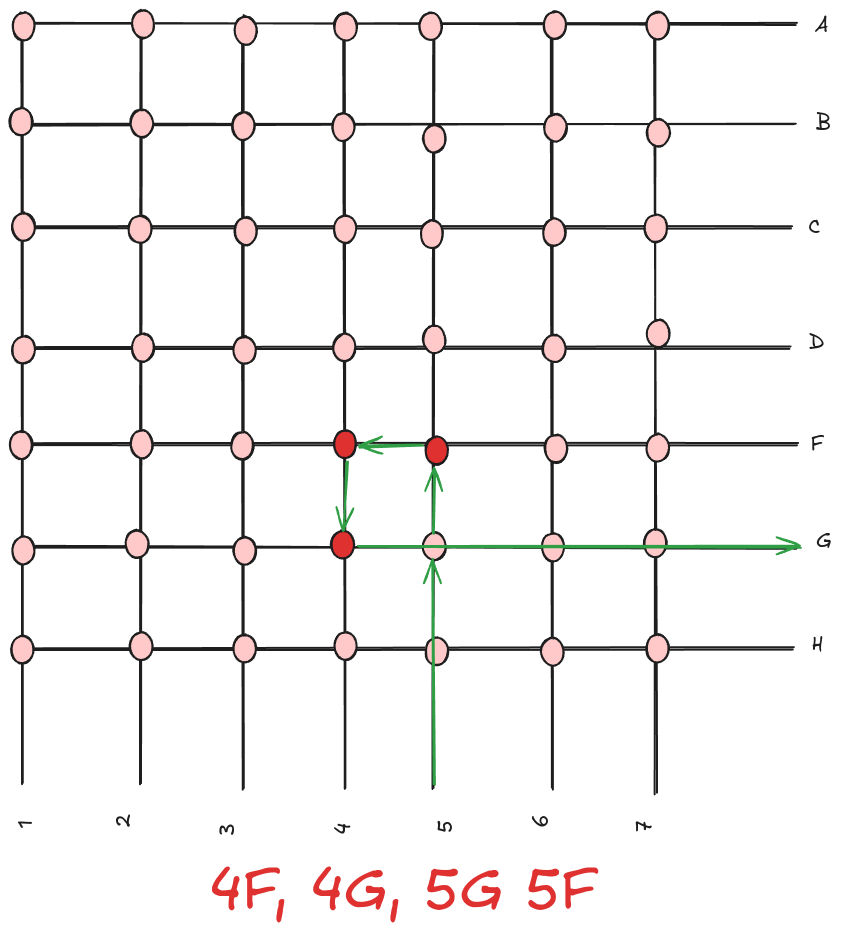
\includegraphics[scale=0.6]{figures/nkr-EX.png}
	\caption{Decoding wrong button press}
\end{figure}

\textbf{N-Key Rollover feature with Diodes}
\begin{figure}[H]
    \centering
    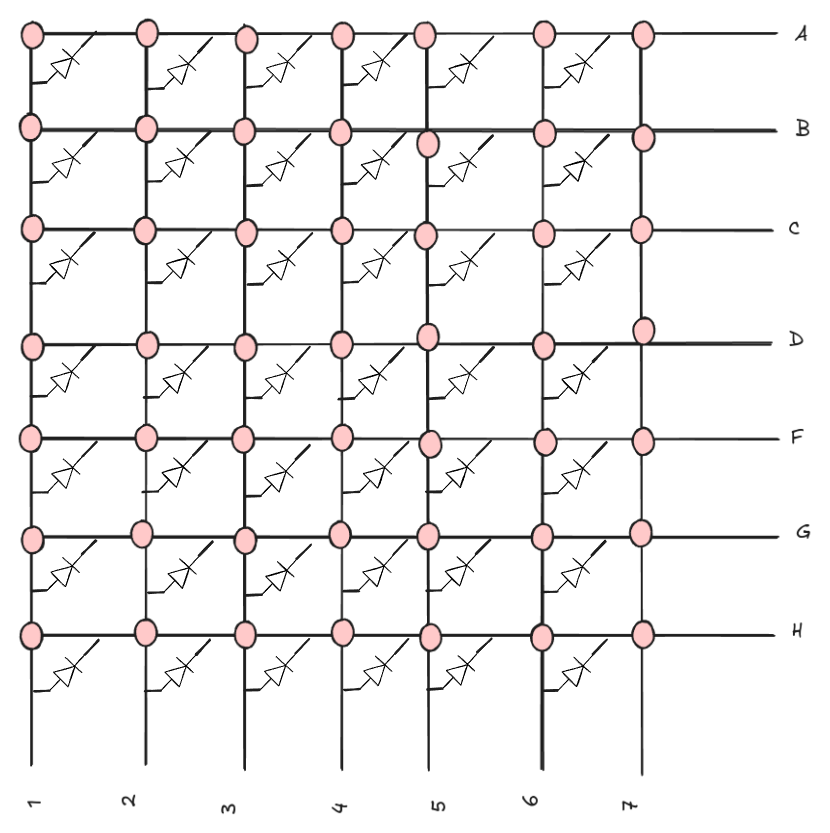
\includegraphics[scale=0.6]{figures/NKRO.png}
    \caption{N-Key Rollover}
\end{figure}

\begin{figure}[H]
	\centering
	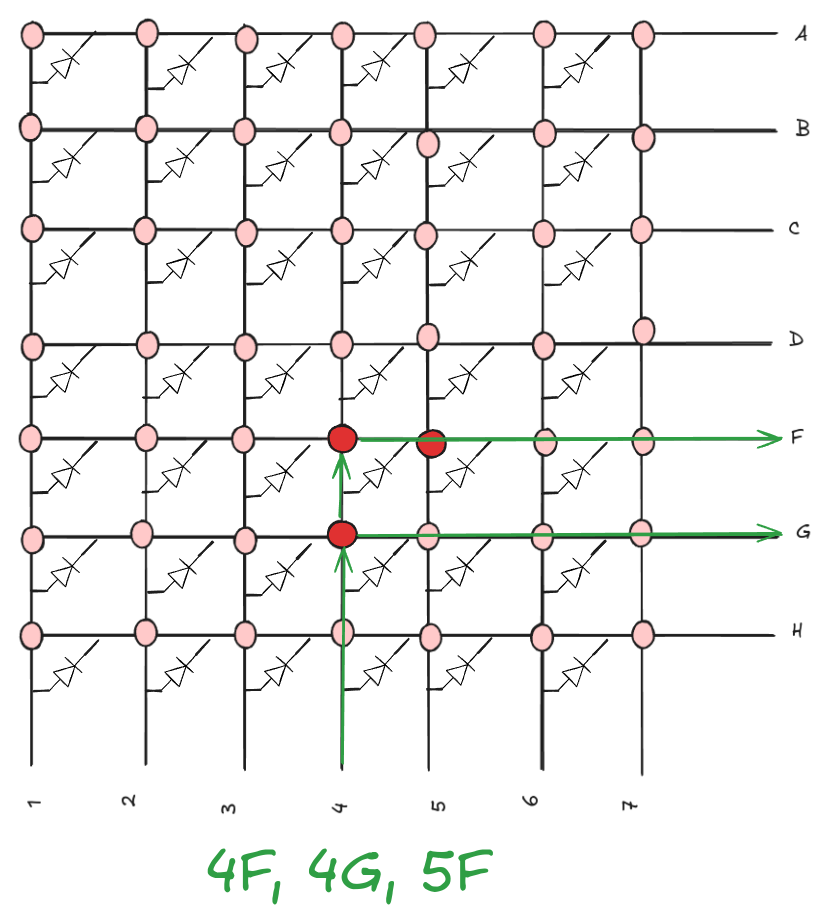
\includegraphics[scale=0.6]{figures/NKRO-EX.png}
	\caption{Multiple keys pressed}
\end{figure}




The keyboard uses a matrix layout, which is an efficient way to manage multiple key inputs with fewer microcontroller pins. In the images, we see an 8x7 matrix (rows A-H, columns 1-7).\\
Scanning Process:\\

The microcontroller scans this matrix by activating one column at a time and reading the state of all rows.
When a key is pressed, it connects a row and column, which the microcontroller detects.\\


\textbf{Ghosting and Its Prevention:}

Ghosting is a problem in simple matrix designs where pressing multiple keys can lead to false key registrations.
Example (Image 1):\\

If keys at 4F, 4G, and 5F are pressed simultaneously, the matrix might also falsely register 5G.\\

\textbf{Solution (Images 2 and 3):}

Diodes are added to each key switch.
These diodes allow current to flow in only one direction, preventing the "phantom" current paths that cause ghosting.
With diodes, when 4F, 4G, and 5F are pressed, 5G is not falsely registered.\\


\textbf{N-Key Rollover (NKRO):}

NKRO allows the keyboard to correctly register any number of simultaneous key presses.\\
Implementation:\\

Each key gets its own diode, ensuring independent registration.
The microcontroller scans the entire matrix rapidly, detecting all pressed keys without conflicts.\\


\textbf{Hardware Components:}

\textbf{Central Microcontroller:}

EFM32BG13 Blue Gecko: This MCU manages all keyboard functions and interfaces with other components.\\

\textbf{Sensors:}

TMP117: Measures temperature, humidity, and pressure, potentially for environmental adaptation or user information.\\
DS3231 RTC Module: Provides accurate timekeeping, useful for time-based functions or logging.\\

\textbf{Display}:

E-Ink Display (800x600, 4.3inch): Offers a low-power way to show keyboard status, settings, or other information.\\

\textbf{Expansion:}

MCP23017 IO Expander: Increases the number of available pins for the key matrix, allowing for more keys or other inputs.\\

\textbf{Power Management:}

Power Management Unit: Manages power distribution and consumption.\\
Li-Ion Polymer Battery: Provides portable power.\\
Energy Harvester: Potentially extends battery life by capturing ambient energy.\\

\textbf{Key Switches and Caps:}

Gateron G Black Pro 2.0 switches: Known for smooth linear action.
Cherry MX key caps: Industry-standard keycaps for customization.\\

\textbf{Additional Inputs:}

Rotary encoders: Provide alternative input methods, possibly for volume control or menu navigation.\\


\textbf{PCB Design:}

4-layer PCB: Allows for more complex routing and better signal integrity.\\
Two versions:\\

Main Module with  all sensors and charging capabilities.\\
Simplified Secondary Module without temperature, humidity, RTC, and LiPo charger.\\


\subsection{Wireless Communication and Software Architecture}

We have made significant progress in defining our wireless communication protocol and software architecture:

\subsubsection{HID Profile Characteristics}
We've detailed the HID (Human Interface Device) profile for our keyboard, including:
\begin{itemize}
    \item Keyboard Input Report: 8-byte structure for key presses
    \item Keyboard Output Report: 1-byte for LED status
    \item Protocol Mode: Supports both Boot and Report protocols
    \item HID Information and Control Point: For device management
    \item Report Map: Defines input/output report formats
\end{itemize}

\subsubsection{Software Architecture}
We've developed a functional software block diagram (Figure \ref{fig:software_diagram}) that outlines the interaction between various software components, including the BLE stack, keyboard matrix scanning, and power management modules.

\begin{figure}[H]
    \centering
    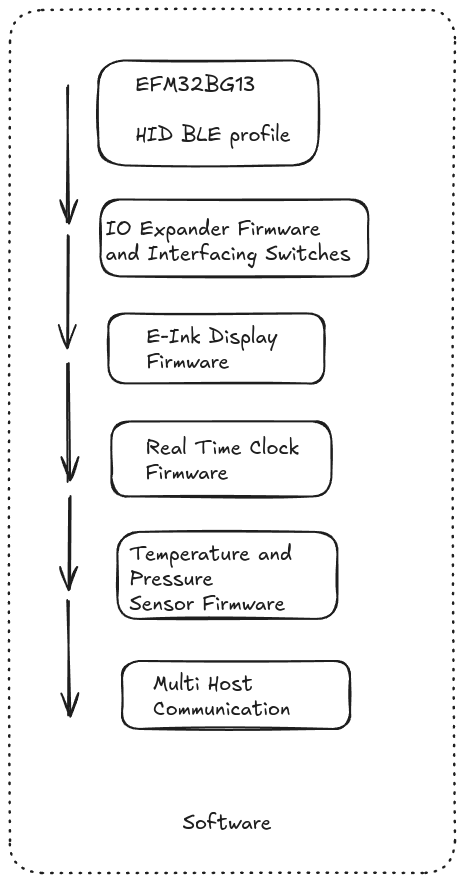
\includegraphics[scale=0.44]{figures/software_diagram.png}
    \caption{Software Block Diagram}
    \label{fig:software_diagram}
\end{figure}

\subsection{Project Management}

We've set up a robust project management system:

\begin{enumerate}
    \item Timeline: We've created a detailed project timeline (Figure \ref{fig:timeline}) to track our progress and milestones.
    
    \item Version Control: Our project is now on GitHub, allowing for better collaboration and code management.
    \begin{itemize}
        \item Project Board: \href{https://github.com/users/parthishere/projects/2}{GitHub Project}
        \item Code Repository: \href{https://github.com/parthishere/Insane-Keyboard}{GitHub Code Repository}
    \end{itemize}
    
    \item Task Tracking: We're using a Kanban board (Figure \ref{fig:kanban}) to manage our tasks and workflow efficiently.
\end{enumerate}

\begin{figure}[H]
    \centering
    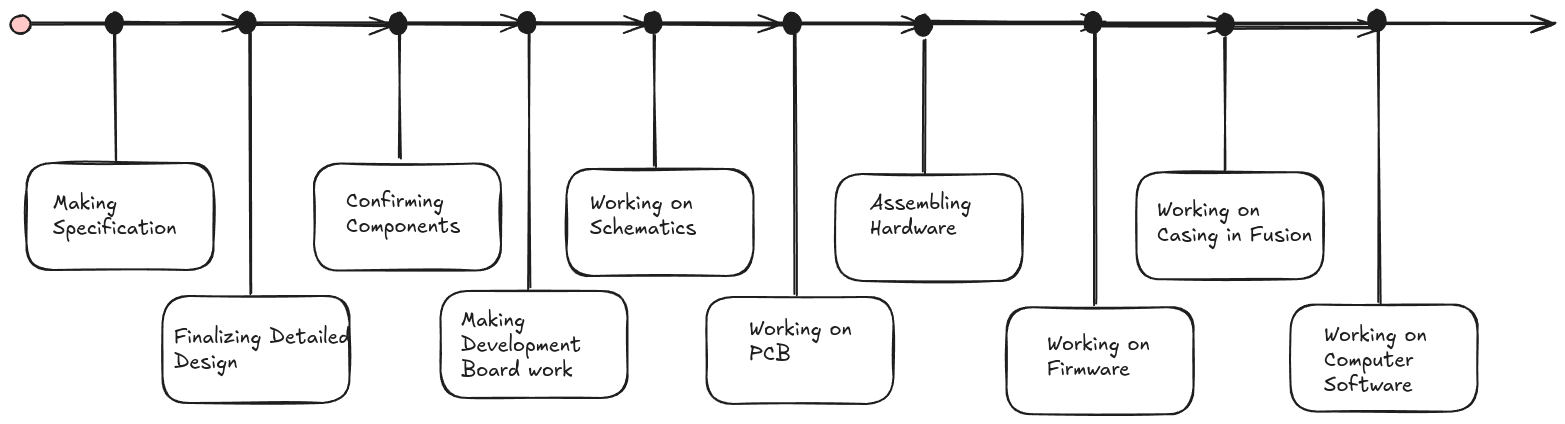
\includegraphics[scale=0.34]{figures/Timeline.png}
    \caption{Project Timeline}
    \label{fig:timeline}
\end{figure}

\begin{figure}[H]
    \centering
    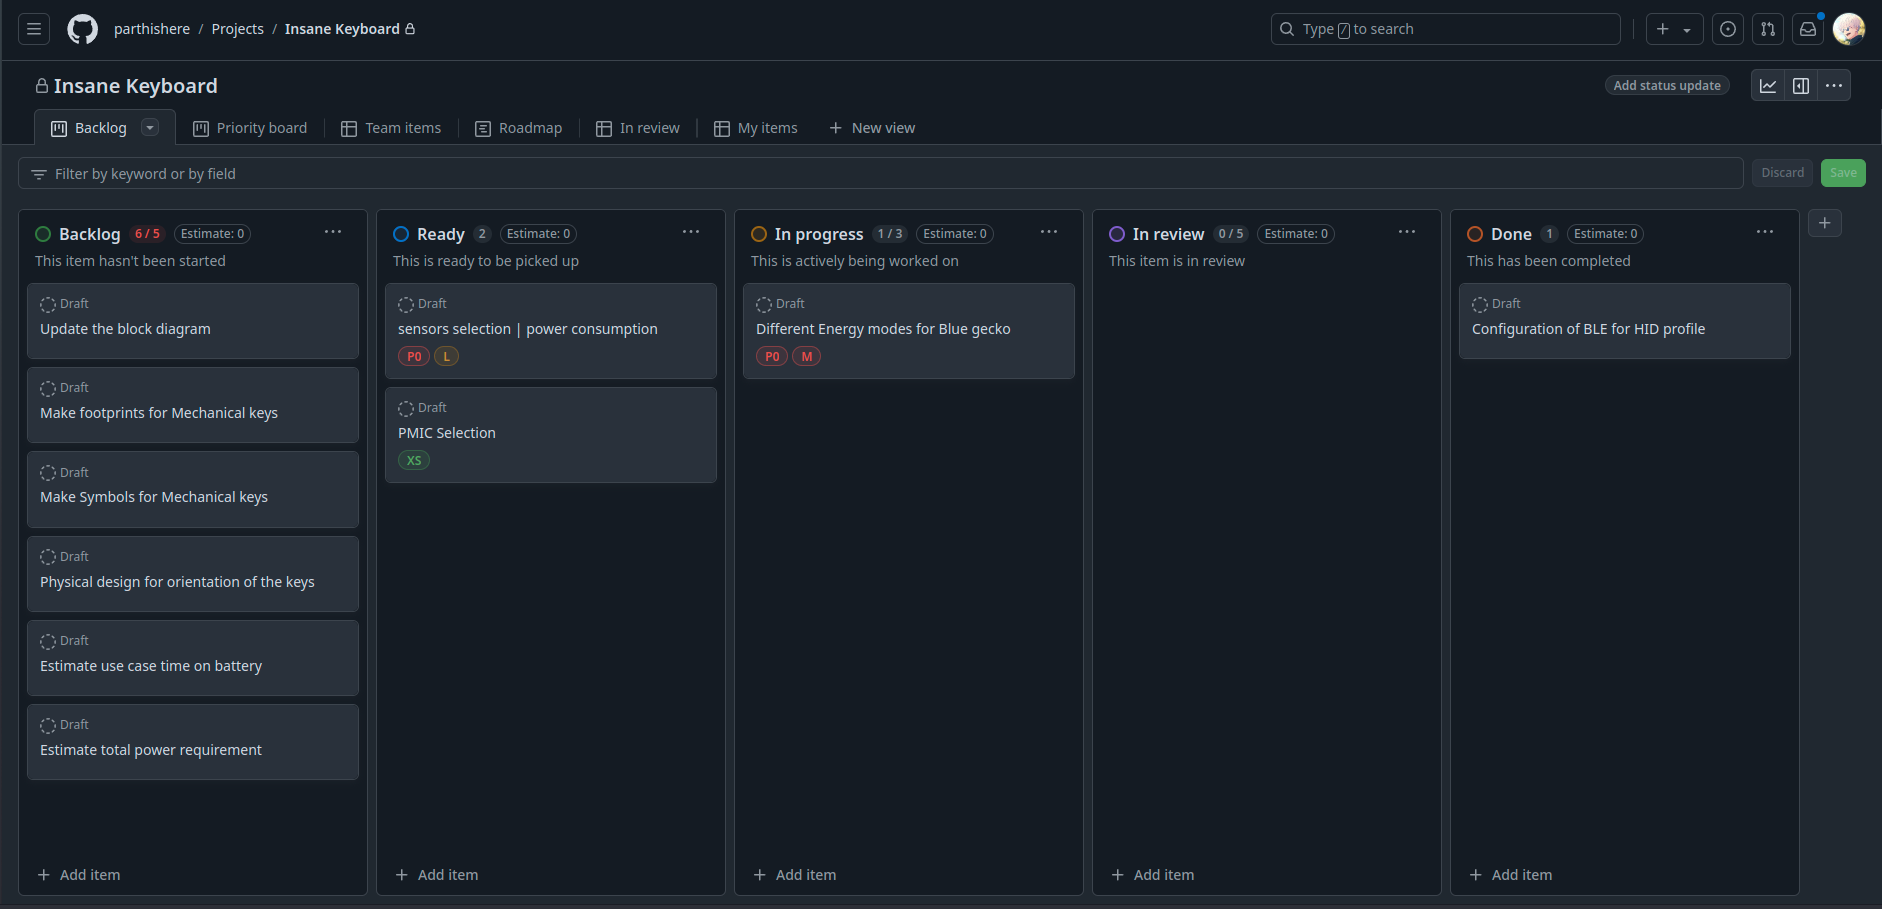
\includegraphics[scale=0.26]{figures/kanban.png}
    \caption{Kanban Board for Task Management}
    \label{fig:kanban}
\end{figure}

\subsection{Energy Analysis and Power Management}

We've conducted initial energy mode analysis and made decisions on power management:

\begin{enumerate}
    \item Energy Calculations: We've performed preliminary calculations (Figure \ref{fig:energy_calc}) to estimate power consumption in various modes.

    \item Energy Harvesting: We've chosen to incorporate a solar panel for energy harvesting, enhancing the keyboard's power autonomy.

    \item Interface Selections:
    \begin{itemize}
        \item Display: SPI interface chosen for faster data transfer
        \item Temperature Sensor and IO Expander: I2C interface for power efficiency
    \end{itemize}

    \item Load Power Management: Implemented a load switch to disable the temperature sensor and display when not in use, reducing standby power consumption.

    \item Multiple Energy Modes: Our design now supports various energy modes to optimize power usage based on the keyboard's current state.
\end{enumerate}

\begin{figure}[H]
    \centering
    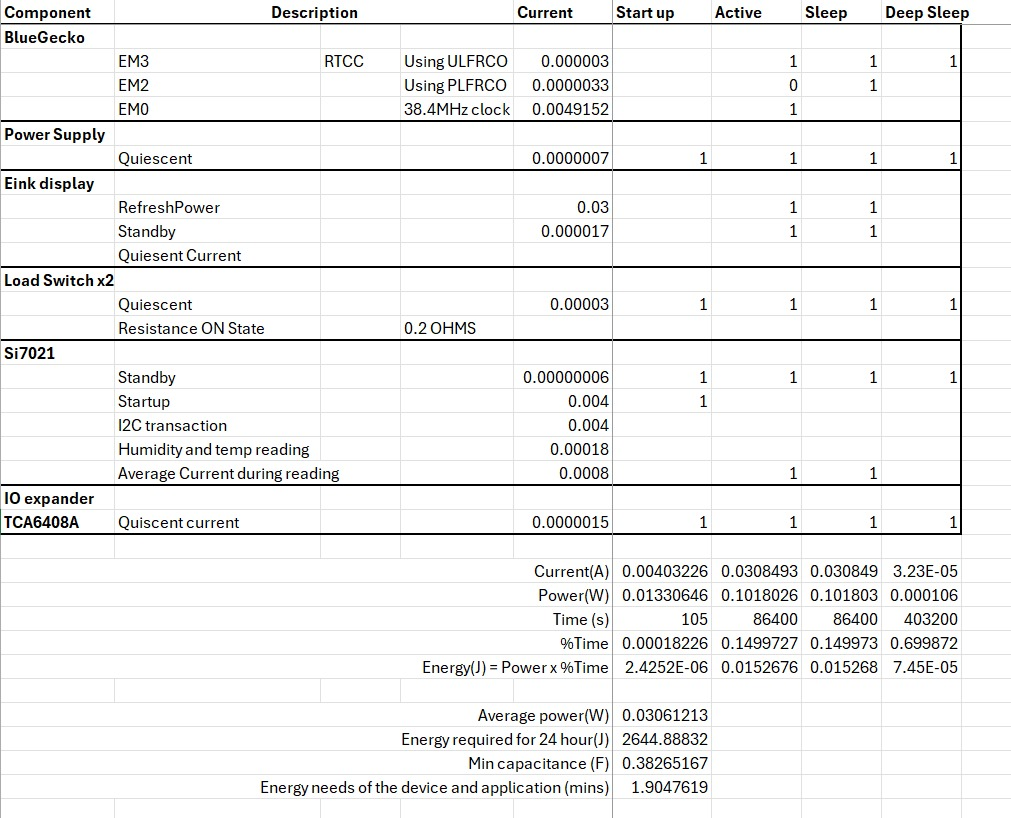
\includegraphics[scale=0.63]{figures/calc.jpeg}
    \caption{Energy Calculations}
    \label{fig:energy_calc}
\end{figure}


\pagebreak

\section{\color{red}Project Update: Week 2}

\subsection{Selection Criteria}
We chose components based on:

\begin{enumerate}
    \item Availability: Multiple suppliers to ensure steady supply.
    \item Power efficiency: Low standby and active currents, multiple power-saving modes.
    \item Documentation: Comprehensive datasheets, application notes, and support.
    \item Sleep modes: Various low-power states with quick wake-up capabilities.
    \item Temperature range: Suitable for varied environments.
    \item EMC/EMI: Built-in interference mitigation.
    \item ongevity: Components not near end-of-life.
    \item Cost: Balanced features and performance with price.
\end{enumerate}


\subsubsection{Chosen Components}


\begin{longtable}{|p{2cm}|p{1.5cm}|p{3cm}|p{1.5cm}|p{6cm}|}
    \hline
    \textbf{Component} & \textbf{Quantity} & \textbf{Function} & \textbf{Interface} & \textbf{DigiKey Part Number} \\
    \hline
    EFR32BG13 & 2 & Microcontroller & - & 
    \href{https://www.digikey.com/en/products/detail/silicon-labs/EFR32BG13P632F512GM32-D/10135852}{EFR32BG13P632F512GM32-D-ND} \\
    \hline
    TCA6408A & 2 & IO Expander & I2C  & 
    \href{https://www.digikey.com/en/products/detail/texas-instruments/TCA6408ARSVR/2044045}{296-24328-1-ND} \\
    \hline
    Waveshare E-ink Display & 1 & Display & SPI  & 
    \href{https://www.waveshare.com/1.54inch-e-paper-module.htm}{External Link} \\
    \hline
    TPS22919 & 1 & Load Switch & -  & 
    \href{https://www.digikey.com/en/products/detail/texas-instruments/TPS22919DCKT/9953066}{296-53421-1-ND} \\
    \hline
    BQ25570 & 2 & PMIC & - & 
    \href{https://www.digikey.com/en/products/detail/texas-instruments/BQ25570RGRT/4430487}{296-37014-1-ND} \\
    \hline
    Battery 1000mAh & 2 & Energy Storage & -  & 
    \href{https://www.digikey.com/en/products/detail/globtek-inc/BL1200P4054481S1PCAC/11201333}{1939-BL1200P4054481S1PCAC-ND} \\
    \hline
    SI7021 & 1 & Temperature and Humidity Sensor & I2C  & 
    \href{https://www.digikey.com/en/products/detail/silicon-labs/SI7021-A20-GMR/5048936}{336-4379-1-ND} \\
    \hline
    Schottky Diodes & 1 & Power Management & -  & 
    \href{-}{Have not decided yet} \\
    \hline
    Gateron G Black Pro 2.0 & 68 & Key Switches & - & 
    \href{https://www.gateron.co/products/gateron-g-pro-2-0-switch-set}{External link} \\
    \hline
    Mechanical Key Hotswap & 68 & Hotswap Sockets & - & 
    \href{https://www.gateron.co/products/gateron-hot-swap-pcb-socket}{External Link} \\
    \hline
    Cherry MX Key Caps & 68 & Key Caps & - & 
    \href{https://www.aliexpress.com/i/3256802573932641.html?gatewayAdapt=4itemAdapt}{External link} \\
    \hline
    Rotary Encoders & 2 & Input Device & - & 
    \href{https://www.digikey.com/en/products/detail/bourns-inc/PEC12R-4222F-S0024/4699283}{PEC12R-4222F-S0024-ND} \\
    \hline
    Solar Panel SM141K06L & 1 & Energy Harvesting & - & 
    \href{https://www.digikey.com/en/products/detail/anysolar-ltd/SM141K06L/9990462}{SM141K06L-ND} \\
    \hline
    \caption{Component List for The Insane Keyboard with DigiKey Part Numbers}
    \label{tab:components}
\end{longtable}


\subsection{Justification for Each Component}

\subsubsection{EFR32BG13 Microcontroller}
\begin{itemize}
    \item Bluetooth 5.0 capable
    \item Energy-efficient: 60 uA/MHz at 40 MHz
    \item Five power modes: 1.4 uA in deep sleep, 20 nA in shutoff
    \item Low-energy peripherals for efficient keyboard scanning
    \item Comprehensive development tools
\end{itemize}


\subsubsection{TCA6408A I/O Expander}
\begin{itemize}
    \item 0.1 uA standby current
    \item 400 kHz I2C interface for quick I/O updates
    \item 8 programmable I/O pins, each sinking 25 mA
    \item Interrupt output for event-driven operation
    \item Chosen over PCA9538 and SX1509 for lower power and simpler programming
\end{itemize}


\subsubsection{Waveshare E-ink Display}
\begin{itemize}
    \item Power used only during updates
    \item Enables dynamic key labeling
    \item SPI interface for fast updates
    \item 200x200 pixel resolution
    \item Preferred over OLED for lower power consumption
\end{itemize}


\subsubsection{TPS22919 Load Switch}
\begin{itemize}
    \item 12 nA quiescent current
    \item 15 us response time
    \item 2A current capacity
    \item 1.5V to 5.5V input range
    \item Built-in protection features
    \item Chosen over TPS22860 and SiP32431 for balanced performance
\end{itemize}


\subsubsection{BQ25570 Power Management IC}
\begin{itemize}
    \item 100 mV to 5.1 V input range
    \item Integrated Maximum Power Point Tracking
    \item 488 nA quiescent current
    \item Built-in boost charger and buck converter
    \item Programmable voltage thresholds
    \item Selected over SPV1050 and ADP5090 for solar power optimization
\end{itemize}


\subsubsection{SI7021 Temperature and Humidity Sensor}
\begin{itemize}
    \item ±0.4°C and ±3\%RH accuracy
    \item 150 nA standby current
    \item I2C interface
    \item 3x3 mm package
    \item 1.9V to 3.6V supply range
    \item Chosen over HDC1080 and BME280 for accuracy and power efficiency
\end{itemize}


\subsubsection{Solar Panel (SM141K06L)}
\begin{itemize}
    \item 42mm x 23mm size
    \item 184 mW maximum output
    \item 3.35V at maximum power point
\end{itemize}


\subsubsection{Battery (1000mAh)}
\begin{itemize}
    \item Size: 2.09" x 1.89" x 0.16"
    \item 525mA charge current, 1.05A discharge current
    \item 3.7V nominal voltage
\end{itemize}


\section{Energy Analysis}
\subsection{Overall Energy Efficiency}
We have made the following assumption for our energy calculations:
The keyboard will be operational 24/7, with the following daily usage pattern:\
8 hours of active use per day
\begin{itemize}
\item 4 hours in active mode
\item 4 hours in sleep mode
\end{itemize}
16 hours in deep sleep mode
\paragraph{Energy Consumption Breakdown}
Based on our calculations, the energy consumption for different operational states is as follows:
\begin{itemize}
\item Start-up: 0.000101970 W
\item Active: 0.0166035556 W
\item Transmit: 0.129140610 W
\item Sleep: 0.000122760 W
\item Deep Sleep: 0.00011187 W
\end{itemize}
\paragraph{Average Power Consumption}
The weighted average power consumption, considering the time spent in each mode, is calculated to be:
\begin{equation}
P_{avg} = 0.003976168 \text{ W}
\end{equation}
This remarkably low average power consumption is achieved through intelligent power management and efficient component selection.
\paragraph{Daily Energy Requirement}
Based on our average power consumption, the total energy required for 24 hours of operation is:
\begin{equation}
E_{daily} = 343.5409345 \text{ J} = 0.095428 \text{ Wh}
\end{equation}
\paragraph{Battery Capacity Calculation}
For sustained operation over a week, we calculated the required battery capacity:
\begin{align*}
E_{weekly} &= 2404.786542 \text{ J} = 0.667996262 \text{ Wh} \
\text{Adjusted Energy} &= \frac{0.667996262}{0.85 \times 0.8} = 0.982347443 \text{ Wh} \
\text{Battery Capacity} &= \frac{0.982347443 \text{ Wh}}{3.7 \text{ V}} \times 1000 = 265.499309 \text{ mAh}
\end{align*}
This calculation takes into account a battery efficiency of 85\% and a maximum depth of discharge of 80\% to ensure long-term battery health.
\paragraph{Energy Harvesting Efficiency}
Our solar panel and power management system are designed to harvest energy efficiently even in low-light indoor conditions. The BQ25570 PMIC, with its Maximum Power Point Tracking (MPPT) capability, ensures optimal energy extraction from the solar panel.
\paragraph{Power Budget Analysis}
\begin{itemize}
\item Average current draw: 1.07464 mA
\item Peak current (during transmission): 39.0296560 mA
\item Quiescent current (deep sleep): 33.9 uA
\end{itemize}
The significant difference between peak and quiescent current underscores the effectiveness of our power-saving modes.
\paragraph{Capacitor Sizing}
To support peak current demands, we calculated a minimum capacitance of:
\begin{equation}
C_{min} = 0.049702103 \text{ F}
\end{equation}
This capacitance ensures stable operation during high-current events while allowing the solar harvesting system to replenish energy during low-power periods.
With an average power consumption of just 3.976 mW and a weekly energy requirement of less than 1 Wh, our keyboard is well-positioned for long-term, self-sustained operation using solar energy harvesting, even in typical indoor environments.
\subsection{Battery and Power Management}
\subsubsection{Power Management IC (PMIC) Selection}
We have selected the BQ25570 PMIC as it provides the necessary features for efficient solar harvesting and battery management. Key features include:
\begin{itemize}
\item Wide input range: 100 mV to 5.1 V, ideal for solar harvesting
\item Integrated Maximum Power Point Tracking (MPPT)
\item Ultra-low quiescent current: 488 nA typical
\item Integrated boost charger and buck converter
\item Programmable voltage thresholds for optimal battery management
\end{itemize}
\subsubsection{Energy Storage Element Selection}
\textbf{Choice: SM141K06L Solar panel}
\begin{itemize}
\item Power Output: 184 mW
\item Voltage at Maximum Power Point (Vmpp): 3.35 V
\item Current at Maximum Power Point (Impp): 55.1 mA
\item Open Circuit Voltage (Voc): 4.15 V
\item Short Circuit Current (Isc): 58.6 mA
\item Size: 42.00mm x 23.00mm x 2.10mm (1.654" x 0.906" x 0.083")
\end{itemize}
Reasons for selection:
\begin{itemize}
\item Significantly higher power output compared to previous options
\item Larger but still manageable size for a keyboard design
\item Higher voltage output, beneficial for power management
\item Good power-to-size ratio
\end{itemize}
Energy Calculations (assuming 8 hours of typical indoor lighting per day):
\begin{flalign*}
&\text{Energy per day} = Power * Time &&\
&\text{Energy per day} = 184 mW * 8 hours  &&\
&\boxed{\text{Energy per day} = 1,472 mWh }&&
\end{flalign*}
Power Density:
\begin{equation*}
\text{Power Density} = \frac{\text{Power Output}}{\text{Area}} = \frac{184 \text{ mW}}{42\text{ mm} \times 23\text{ mm}} = \boxed{0.191 \text{ mW/mm²}}
\end{equation*}
\subsection{Energy Requirements Analysis}
\subsubsection{Unregulated Supply Performance}
Constant Power Case:
\begin{itemize}
\item Regulated power supply providing power for microcontroller and sensors which require input voltage kept in limited range.
\item As voltage out of energy source drops from Vworking to Vmin, current increases to keep power through supply constant.
\end{itemize}
\subsubsection{Peak and Average Current Use Cases}
We have analyzed the current requirements for each component in our system under both peak and average use conditions. Table \ref{tab:current_requirements} summarizes these findings:
\begin{table}[H]
\centering
\begin{tabular}{|l|c|c|}
\hline
\textbf{Component} & \textbf{Peak Current (A)} & \textbf{Average Current (A)} \\
\hline
Temperature Sensor & 0.004 & 0.00071424 \\
\hline
E-ink Display & 0.008 & 8.05558E-05 \\
\hline
MCU & 0.0393152 & 0.000115536 \\
\hline
PMIC & 0.0000009 & 0.0000009 \\
\hline
Load Switch & 0.0000201 & 0.0000201 \\
\hline
IO Expander & 0.0000015 & 0.0000015 \\
\hline
\textbf{Total} & 0.0513377 & 0.000932832 \\
\hline
\end{tabular}
\caption{Component Current Requirements}
\label{tab:current_requirements}
\end{table}
\subsubsection{Total Energy Required Between Charging}
Given:
\begin{itemize}
\item Battery Capacity: 1000 mAh
\item Assumed Battery Voltage: 3.7 V (typical for Li-ion)
\item Daily Energy Consumption: 343.5409345 J
\end{itemize}
Calculations:
\begin{enumerate}
\item \textbf{Convert Battery Capacity to Joules:}
\begin{equation}
\text{Energy (J)} = \text{Capacity (mAh)} \times \text{Voltage (V)} \times 3.6
= 1000 \times 3.7 \times 3.6 = 13,320 \text{ J}
\end{equation}
\item \textbf{Calculate Number of Days:}
\begin{equation}
\text{Days} = \frac{\text{Total battery energy}}{\text{Daily energy consumption}}
= \frac{13,320 \text{ J}}{343 \text{ J/day}} \approx 38.83 \text{ days}
\end{equation}
\item \textbf{Convert to Weeks:}
\begin{equation}
38.83 \text{ days} \approx 5.55 \text{ weeks}
\end{equation}
\end{enumerate}
\subsubsection{Recharge Time Calculation}
We are using a 1000mAh battery with a 0.5C charging rate:
\begin{itemize}
\item Theoretical charging current: 0.5C = 500mA
\item BQ25570 PMIC maximum charging current: 230mA (typical)
\end{itemize}
Since the PMIC can't provide 500mA, it will charge at its maximum rate of 230mA.
\begin{equation}
\text{Estimated charging time} = \frac{\text{Battery Capacity}}{\text{Charging Current}}
= \frac{1000\text{mAh}}{230\text{mA}} \approx 4.35 \text{ hours}
\end{equation}


\subsection{Supercapacitor vs Battery Comparison}

In considering energy storage options for our keyboard, we evaluated a 4F Vishay supercapacitor against our chosen 1000mAh Li-ion battery. This analysis is crucial for optimizing the keyboard's performance and longevity.

\subsubsection{Energy and Power Density}

\begin{itemize}
    \item \textbf{Battery:} Our 1000mAh Li-ion battery at 3.7V stores approximately 3.7Wh of energy.
    \item \textbf{Supercapacitor:} The 4F Vishay supercapacitor, assuming a 2.7V rating, stores about 0.004Wh.
\end{itemize}

The battery clearly outperforms in energy density, crucial for our keyboard's long-term operation between charges.

\subsubsection{Peak Current Handling}

\begin{itemize}
    \item \textbf{Battery:} Our battery can handle discharge currents up to 1.05A.
    \item \textbf{Supercapacitor:} Supercapacitors generally excel in delivering high peak currents.
\end{itemize}

While both can meet our peak current requirement of 39.0296560 mA, the supercapacitor might provide better performance for rapid, high-current events.

\subsubsection{Temperature Range}

\begin{itemize}
    \item \textbf{Battery:} Typical Li-ion batteries operate effectively between 0°C and 45°C.
    \item \textbf{Supercapacitor:} Vishay supercapacitors often have a wider operating range, potentially from -40°C to 65°C.
\end{itemize}

The supercapacitor's wider temperature range could be advantageous, but our keyboard's expected operating range (0°C to 50°C) is well within the battery's capabilities.

\subsubsection{Cycle Life and Longevity}

\begin{itemize}
    \item \textbf{Battery:} Li-ion batteries typically last for 500-1000 charge cycles.
    \item \textbf{Supercapacitor:} Supercapacitors can often withstand 100,000+ charge cycles.
\end{itemize}

The supercapacitor significantly outperforms in cycle life, which could be beneficial for frequent charge-discharge scenarios.

\subsubsection{Self-Discharge and Shelf Life}

\begin{itemize}
    \item \textbf{Battery:} Li-ion batteries have a relatively low self-discharge rate, losing about 5-10\% of their charge per month.
    \item \textbf{Supercapacitor:} Supercapacitors typically have higher self-discharge rates, potentially losing significant charge within days or weeks.
\end{itemize}

The battery's lower self-discharge rate is preferable for our keyboard, which may have periods of inactivity.

\subsubsection{Charging Characteristics}

\begin{itemize}
    \item \textbf{Battery:} Our battery charges at 525mA, taking about 2 hours for a full charge.
    \item \textbf{Supercapacitor:} Supercapacitors can be charged much faster, potentially in seconds or minutes.
\end{itemize}

The supercapacitor's rapid charging could be beneficial for quick top-ups, but may not be necessary given our solar charging setup.

\subsubsection{Size and Weight}

\begin{itemize}
    \item \textbf{Battery:} Our battery measures 2.09" x 1.89" x 0.16".
    \item \textbf{Supercapacitor:} The 4F Vishay supercapacitor is likely smaller and lighter.
\end{itemize}

While the supercapacitor might offer space savings, our chosen battery fits well within our keyboard's design constraints.
For our keyboard application, the Li-ion battery remains the preferred choice.



\subsection{PCB Design Progress}
We've completed footprint creation for most components, with the following exceptions:

Solar Panel: Recently added, footprint pending
0603 components: Footprints for resistors and MLCC capacitors still needed

\subsubsection{Footprint Generation}
Footprints:

\begin{figure}[H]
    \centering
    \begin{tabular}{cc}
        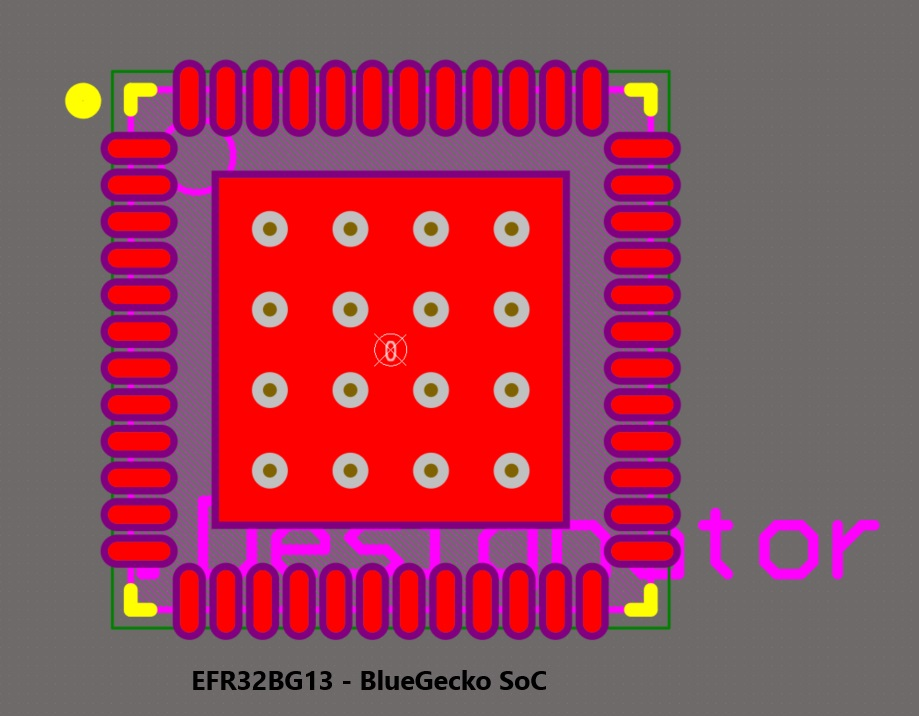
\includegraphics[width=0.40\linewidth]{figures/BlueGecko.jpg} &
        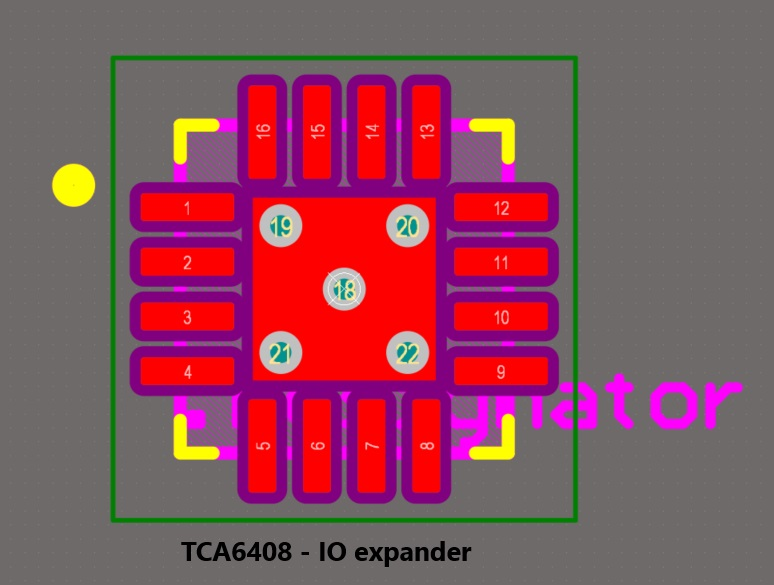
\includegraphics[width=0.40\linewidth]{figures/IO expander.jpg} \\
        BlueGecko EFR32BG13 QFN48 package & IO expander \\
        
        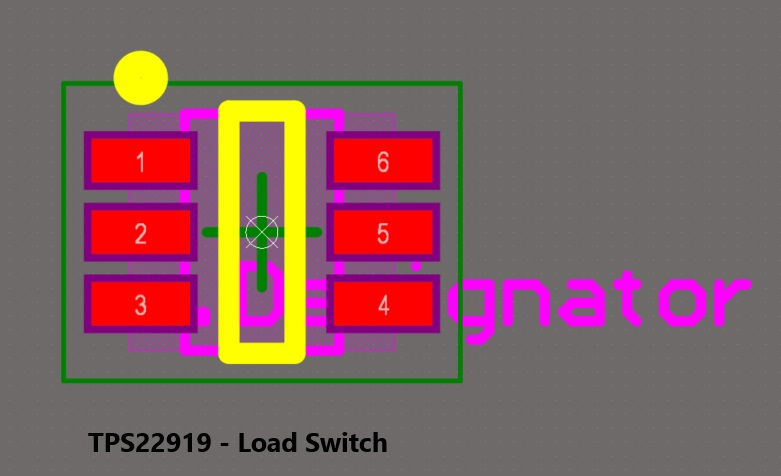
\includegraphics[width=0.40\linewidth]{figures/Loadswitch.jpg} &
        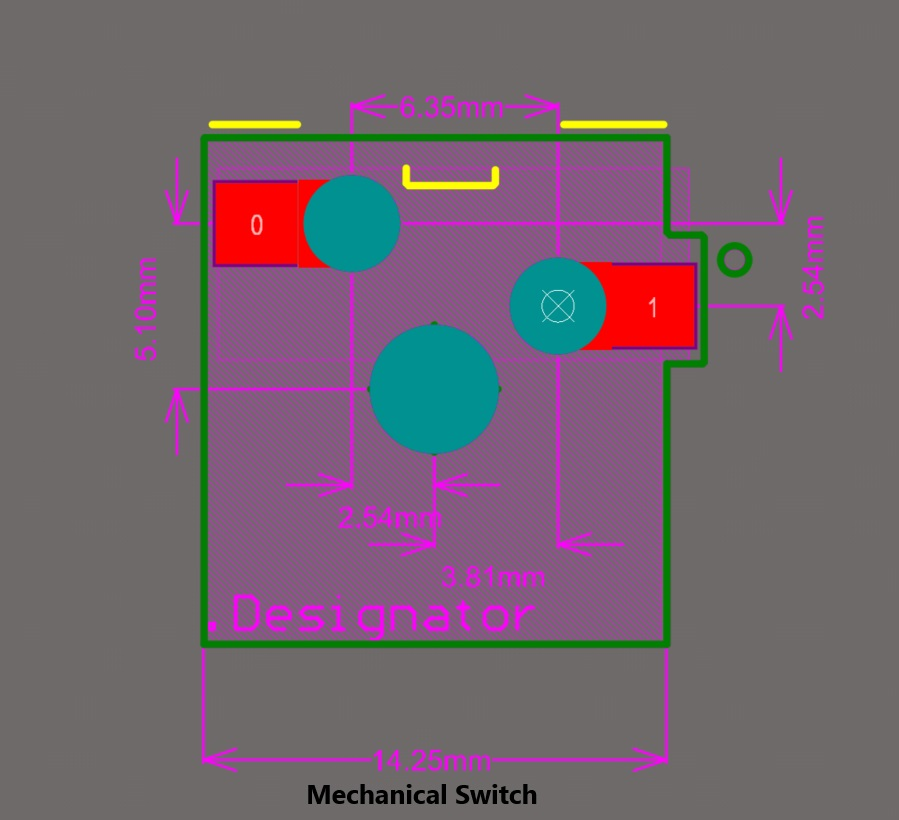
\includegraphics[width=0.40\linewidth]{figures/Mechanical Switch.jpg} \\
        Loadswitch & Mechanical switch \\
        
        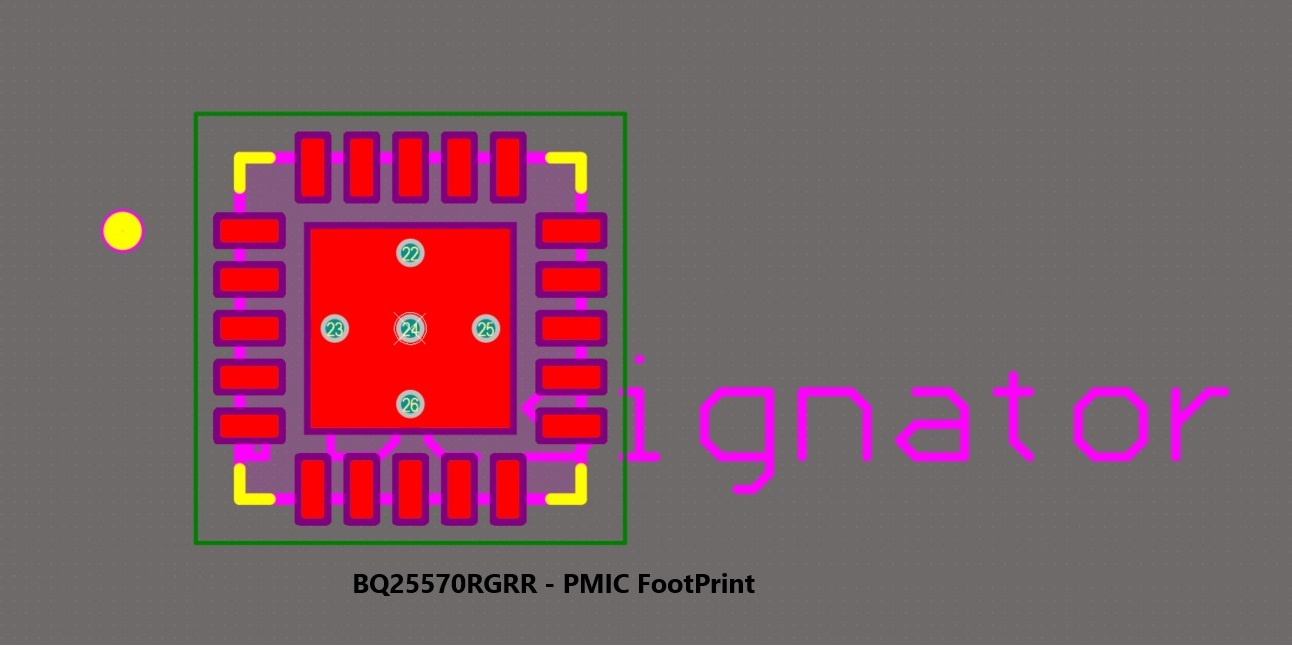
\includegraphics[width=0.40\linewidth]{figures/PMIC.jpg} &
        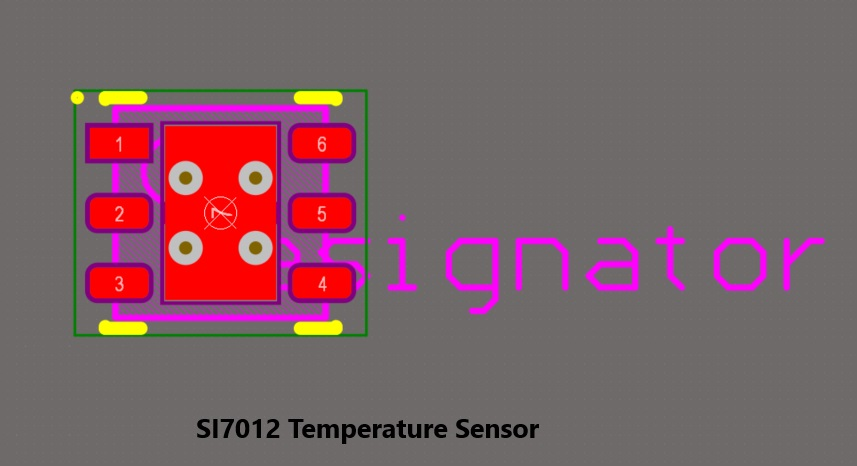
\includegraphics[width=0.40\linewidth]{figures/Temperature sensor.jpg} \\
        PMIC & Temperature Sensor
    \end{tabular}
    \caption{Component Footprints}
    \label{fig:component_footprints}
\end{figure}

\subsubsection{Power Supply Considerations}
For components requiring a stable input voltage:

A regulated power supply will be used
As the energy source voltage decreases, current will increase to maintain constant power

\subsection{Mechanical Design}
\subsubsection{Dimensions}

Left unit: 165mm x 120mm x 35mm\\
Right unit: 175mm x 120mm x 35mm

\subsubsection{Material}
Carbon fiber-filled Nylon selected for construction
\subsubsection{Operating Conditions}

Temperature range: 0°C to 50°C\\
Voltage range: 
\begin{figure}[H]
	\centering
	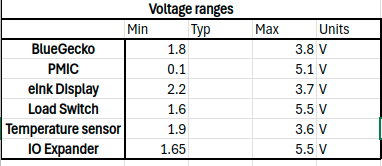
\includegraphics[scale=0.6]{figures/vr}
	\caption{Voltage Range}
\end{figure}














\subsection{Project Progress and Future Plans}
\subsubsection{Recent Updates}
\begin{itemize}
    \item Added solar panel for energy harvesting
    \item removed Supercapacitor
    \item Added links to components
    \item created Libraries
\end{itemize}
\begin{figure}[H]
	\centering
	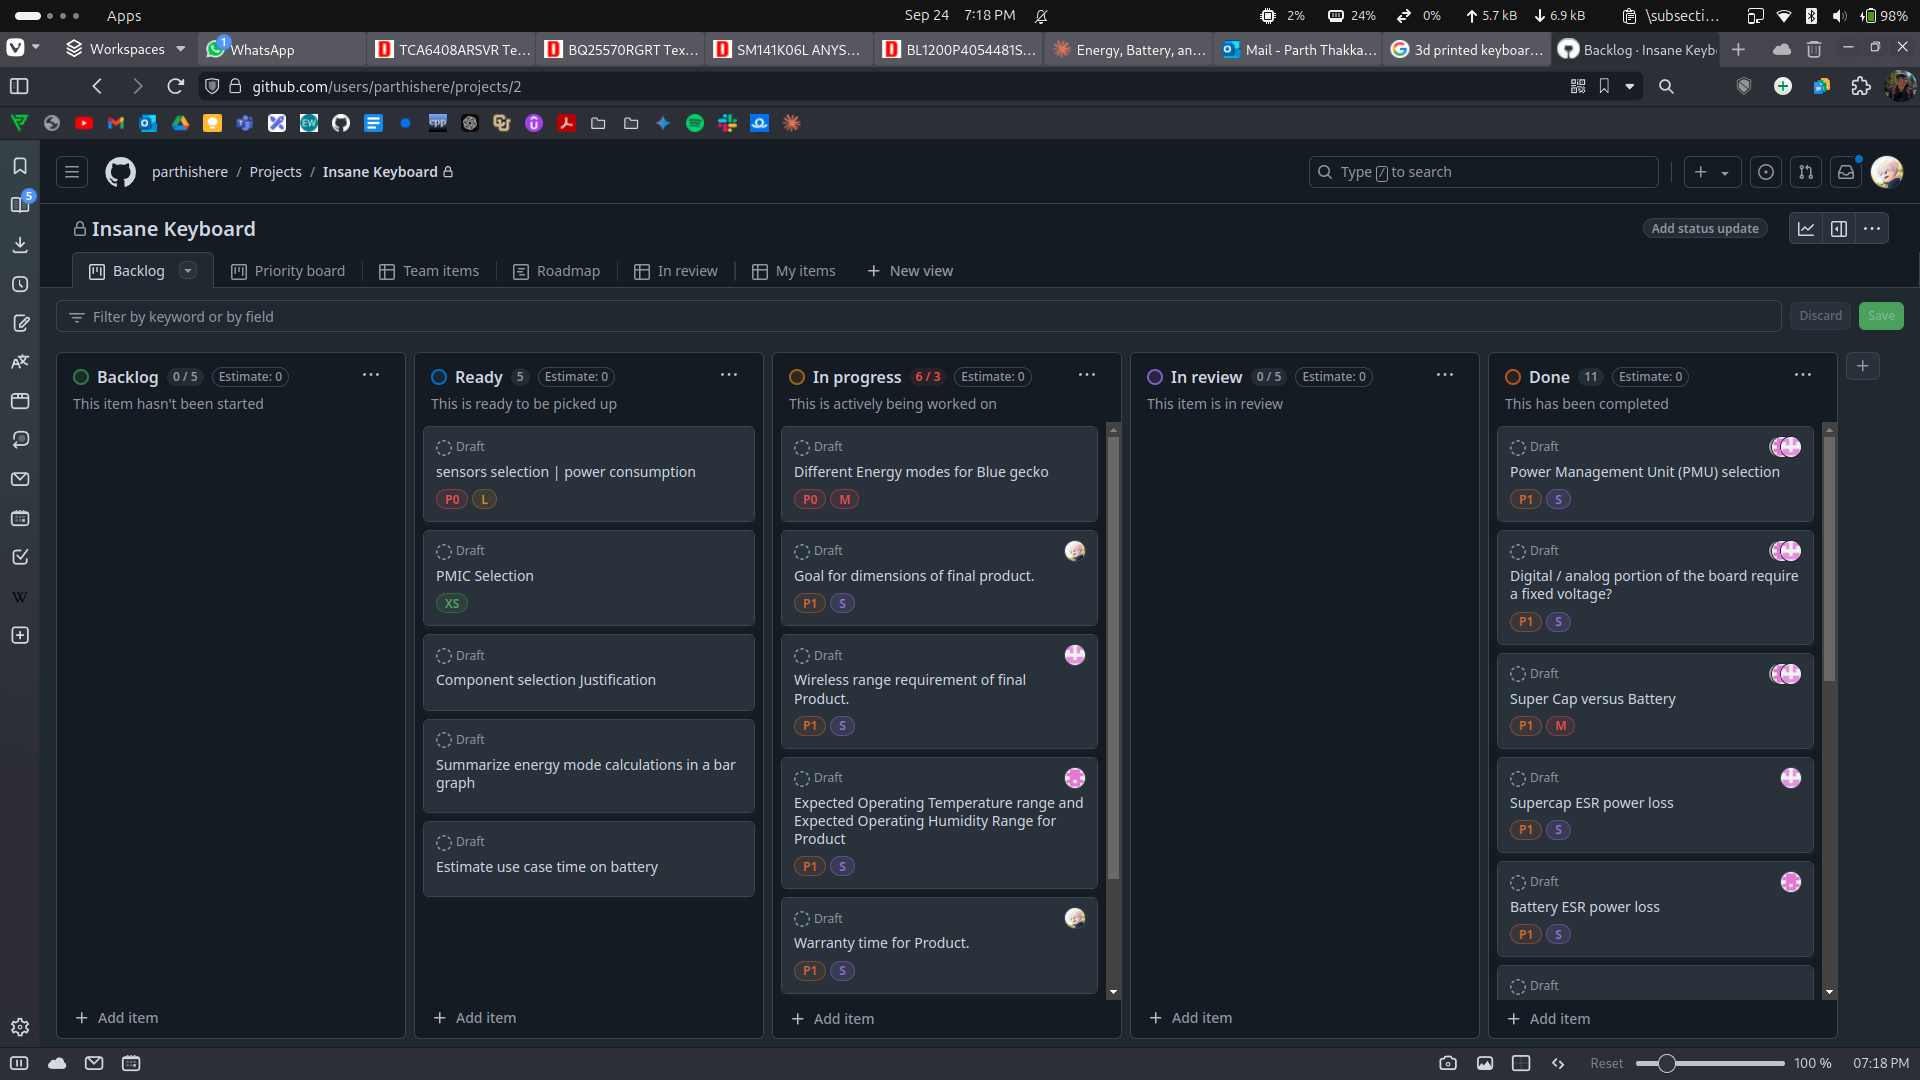
\includegraphics[scale=0.22]{figures/kanban_2.png}
	\caption{Kanban for update 2}
\end{figure}


\subsubsection{Upcoming Tasks}
\begin{enumerate}
    \item Component Selection:
    \begin{itemize}
        \item Choose appropriate decoupling capacitors
    \end{itemize}
    \item Design Refinement:
    \begin{itemize}
        \item Optimize key size and spacing for ergonomics
        \item Finalize keyboard layout
    \end{itemize}
    \item Prototyping Preparation:
    \begin{itemize}
        \item Design 3D case model using Fusion 360
        \item 3D print prototype case
    \end{itemize}
\end{enumerate}

\begin{figure}[H]
	\centering
	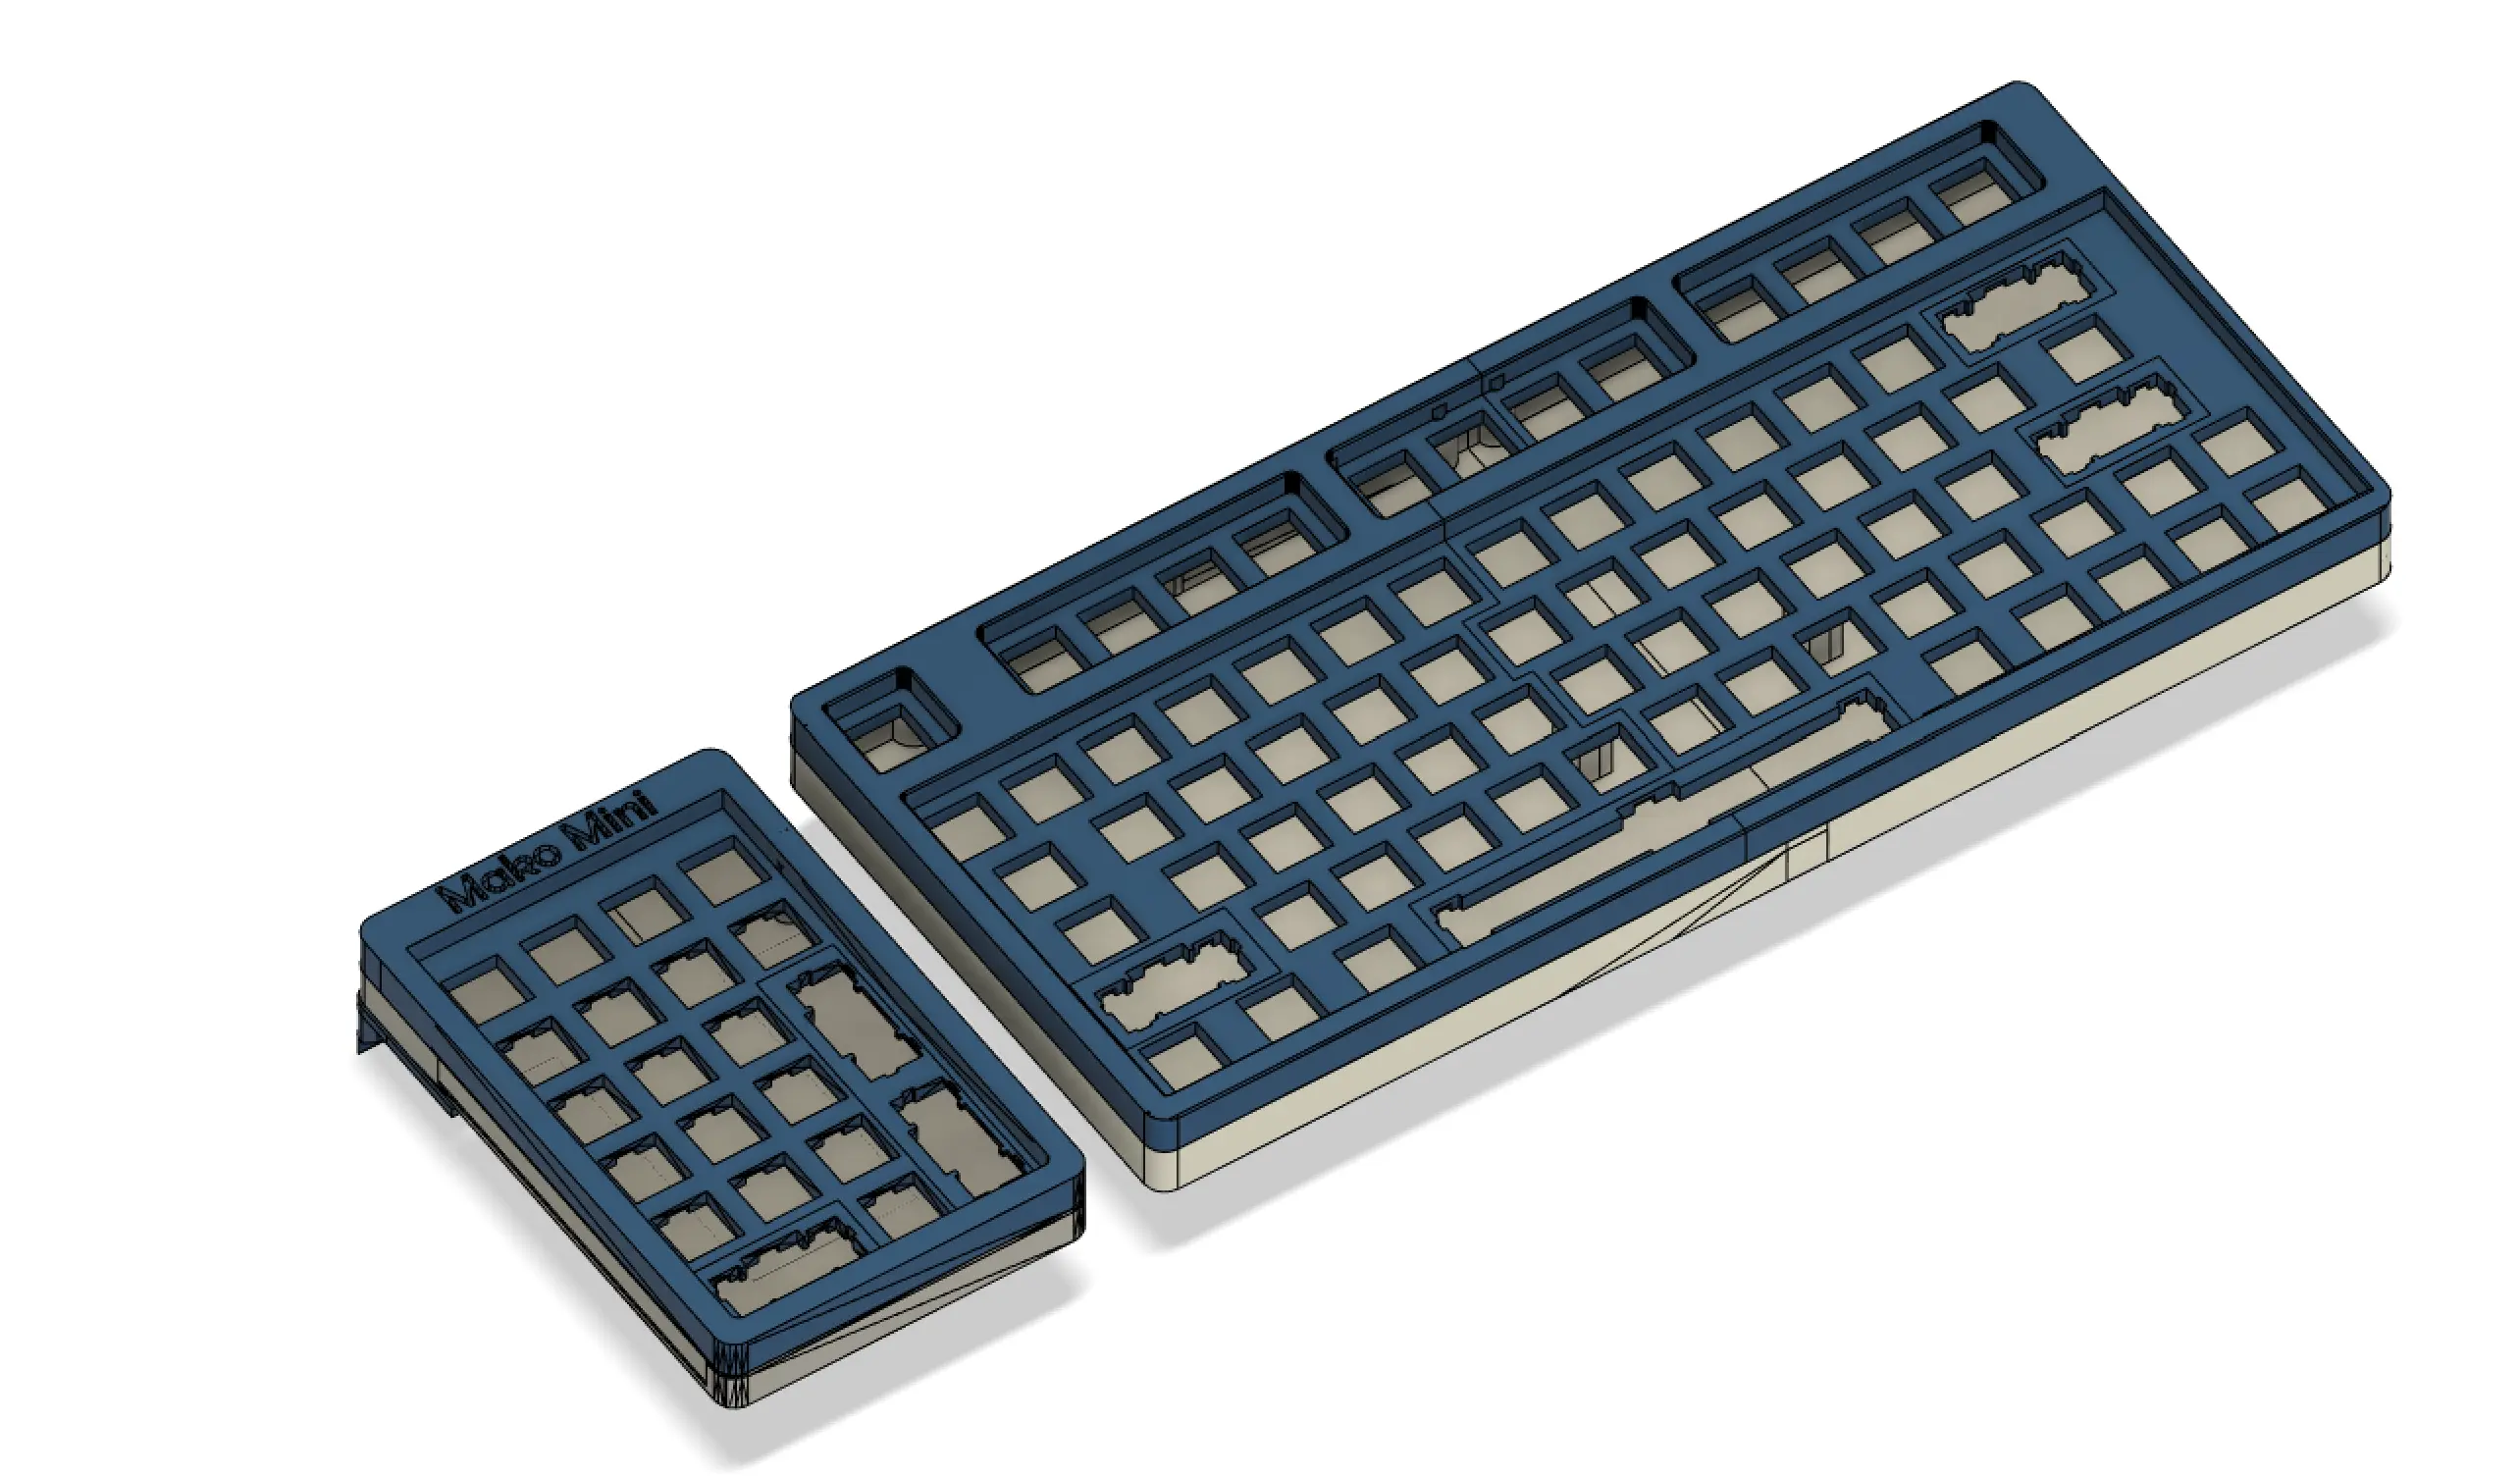
\includegraphics[scale=0.17]{figures/3d_print_fusion.png}
	\caption{Design a Case and PCB}
\end{figure}

\pagebreak


\hrule






%---------------------------------------------------------------------------
\end{document}
-
